\documentclass[12pt]{article}
\usepackage[utf8]{inputenc}
\usepackage{amsmath,amssymb,hyperref,array,xcolor,multicol,verbatim,mathpazo}
\usepackage[normalem]{ulem}
\usepackage[pdftex]{graphicx}
\usepackage{fullpage}
\usepackage{import}
\usepackage{adjustbox}
\usepackage{booktabs}
\usepackage{bbm}
\usepackage[font=normalsize,labelfont=bf]{caption}
%\captionsetup{justification=raggedright,singlelinecheck=false}
\usepackage{subcaption}

\usepackage[backend=biber,style=authoryear,
sorting=ynt,citestyle=authoryear]{biblatex}
\addbibresource{papercitations.bib}
\usepackage{setspace}
\onehalfspacing
\addtolength{\skip\footins}{2pc plus 5pt}

\usepackage{geometry}
 \geometry{,
 left=25.4mm,
 top=25.4mm,
 right=25.4mm,
 bottom=25.4mm
 }
 

\title{Labor Markets and Technological Change: Evidence from Electronic Health Records}
\author{Hanna Glenn}
%\date{\today}

\DeclareLabeldate[online]{%
  \field{date}
  \field{year}
  \field{eventdate}
  \field{origdate}
  \field{urldate}
}
\usepackage{times}
\begin{document}

\maketitle

\begin{abstract}
    Technology adoption in health care is of great importance to policy makers as some technologies are expected to radically improve the U.S. health care system. However, some new technologies can be burdensome for physicians and lead to frustration. I add to our understanding of a new technology's affect on workers by investigating changes in physician behavior as a result of a major technology shift in U.S. hospitals, electronic health records (EHRs). I treat EHR implementation in hospitals as an exogenous treatment to physicians within the hospital (hospitalists), and estimate average group time treatment effects on various labor market outcomes. I find that hospitalists are 10\% more likely to retire, and at least 15\% more likely to work in an office due to EHRs. Further, those exposed to EHRs see more patients due to the technology. These results point to unintended consequences of rapid technology implementation, but also indicate potential productivity gains for those who embrace the technology.
\end{abstract}

\vspace{1.5cm}

\section{Introduction}
For decades technological innovation has brought about changes to production in the economy through adjustments in wages, demand for labor, and other aspects of labor markets. Still, advancement of modern technology is rapid, and it is not clear how policymakers should be involved in the implementation of new technologies. This is particularly important in health care, where new technologies can impact patient outcomes. A recent technology roll-out that altered the US health care system dramatically was the electronic health record (EHR). Medical entities nationwide implemented EHRs rapidly from 2008-2015, with the percentage of hospitals with basic EHR capability increasing from 9 percent to 84 percent. Since many physicians working in hospitals were exposed to this technology in a concentrated time, this is an opportune setting to investigate the relationship between rapid technology implementation and individual labor market behaviors. In this paper, I investigate the effect of EHR adoption in hospitals on several behaviors of physicians working in hospitals. 

EHRs are computer systems that house digital medical records and sometimes have additional functionalities. EHRs have become increasingly relevant in the US since 2009, when the Health Information Technology for Economic and Clinical Health (HITECH) Act was passed to subsidize hospitals and practices who implement and ``meaningfully'' use an EHR (\cite{hitech}).\footnote{According to Quatris Healthco, meaningful use standards proceeded in three stages over time. In Stage 1 (2010), MU focused on data capturing and sharing. In Stage 2, which began in late 2012, MU extended to using EHRs for patient incorporation and using the technology as a helper in care. Stage 3 went from 2014-2016 and focused on making data accessible across hospitals (\cite{meanuse})} President Obama stated in 2009, “To improve the quality of our health care while lowering its cost, we will make the immediate investments necessary to ensure that, within five years, all of America’s medical records are computerized.” (\cite{presquote}). The push for EHR use stemmed from a widespread expectation that EHRs would improve quality of health care while decreasing costs, the gold standard in health policy. For example, a 2005 study estimated hundreds of billions of dollars saved if health information technology were to be fully implemented (\cite{hillestad2005}).

Physicians, as the primary users of EHRs, play an important role in whether the expected benefits come to fruition. Daily tasks change drastically when a new system is put in place; some physicians reported that when using EHRs they are less satisfied with their job and have higher stress levels. Senior physicians in particular “loathe the cumbersome, time-consuming data entry that comes with using EHR.” (\cite{CollierBurnout}). When looking solely at hospitalists, 63\% of survey respondents found EHRs time consuming and inefficient (\cite{czernik2022hospitalist}). The frustration of a new technology raises the cost of working in settings that use it, which may lead physicians on the margin to make behavioral changes such as exiting the labor market altogether or shifting towards alternative work settings. However, the extent to which this frustration actually imposes a meaningful cost is unknown, making physician response an empirical question. For a hospitalist, the hospital's decision to adopt an EHR is plausibly exogenous. Thus, I use a difference-in-differences research design to estimate the effect of EHR adoption on hospitalist labor market choices: (1) exiting clinical environments, measured based on no future claims, (2) substituting hospital work for office work, measured by the location of claims, and (3) productivity, measured by the number of patients seen and claims filed per patient.

While hospitalists create an ideal setting to answer this question econometrically, they are also important in their own right. The Bureau of Labor Statistics estimates approximately 44,000 physicians employed as hospitalists in the US, and studies estimate that 75\% of hospitals employ hospitalists (\cite{bls}, \cite{healthecareers_2022}). Further, one third of Medicare admissions are seen by a hospitalist (\cite{messler2015history}). I construct a panel of hospitalists spanning from 2009-2017. Using Centers for Medicare and Medicaid Services (CMS) Shared Patient Data, I identify the hospital affiliation of each hospitalist. Then, I use the American Hospital Association (AHA) Survey to determine EHR adoption status, and thus connect hospitalists to EHR exposure. Finally, I use Medicare Data on Provider Practice and Specialty (MD-PPAS) for information on the patients seen by each hospitalist. The independent variable of interest is binary, capturing exposure to an EHR.\footnote{While there are ample nuances to EHRs, I abstract away from these as I focus on the inital shock of a new technology.} I estimate group-time treatment effects of EHR exposure on the physician decisions defined above.

This paper contributes to our understanding of the effects of health information technology. There is robust empirical research examining the effect of EHRs on patient outcomes and hospital costs, but these studies largely use data prior to the subsidization of meaningful EHR use. Despite a large number of case studies that find generally positive effects, i.e., improved patient outcomes and decreased cost (surveyed in \cite{Buntin2011TheResults}), economic work has found a mixture of results: outcomes for median patients do not change as a result of EHRs (\cite{Agha2014TheCare}, \cite{McCullough2016HealthCoordination}, \cite{Meyerhoefer}) while newborns and severe patients experience improvement in health outcomes (\cite{Miller2009}, \cite{Freedman2015}, \cite{McCullough2016HealthCoordination}), and hospital costs only decrease 6 years after implementation, if at all (\cite{Agha2014TheCare}, \cite{dranove2014trillion}). A number of case studies consider the effect of EHRs on productivity. One study finds that nursing home productivity increases after adopting health IT (\cite{Hitt2016}), but another finds that physician productivity decreases by 11 percent due to EHRs being adopted in primary-care sites (\cite{Meyerhoefer}). There is still much to be learned about EHRs effects on health care, specifically related to labor supply (\cite{NBERw29218}). 

I expand this literature first by considering individual physician labor market decisions as an outcome, which, to my knowledge, has not yet been examined. Further, I consider the primary time period in which EHRs were rapidly implemented. This provides sufficient variation in the timing of adoption and ensures the EHRs are meaningful and are likely affecting physicians' daily life. Similarly to past studies, I consider EHR implementation as a treatment variable in a difference-in-differences framework. I improve on this strategy by estimating average group time treatment effects for multiple years after implementation, which avoids common problems that arise in typical two way fixed effects estimation with heterogeneous effects.  

Early research on the inputs to physician retirement decisions found that the most influential factors are personal and financial matters, and that physicians care about their work environment (specifically in the context of managed care organizations), but do not necessarily retire early because of it (\cite{Bahrami2002}). Contrary to this result, I find that EHR implementation led to a 20\% increase in the likelihood of exiting clinical settings for hospitalists of age 60 plus. Physicians less than 60 were 7\% more likely to exit, possibly pointing to career switching. Limiting the sample to those who remained in clinical settings, I find that hospitalists were 30\% more likely to start seeing patients in an office setting at the time of exposure. Finally, I find that EHRs lead to a patient count increase of at least 20 patients per year, and the increase is large enough that it is not entirely driven by a redistribution of patients from those who left clinical settings. 

Two key assumptions underlie the main analysis. First, I assume that hospitalists are constrained to use the technology implemented in their work setting. Second, I assume the decision for hospitals to implement EHRs is exogenous to individuals. That is, a hospitalist employed by the hospital does not choose their own EHR exposure. My main findings are not sensitive to a plethora of robustness checks, and the results suggest that there was a surge of experienced hospitalists who left both clinical settings altogether and the hospitals where the EHR was deployed. Thus, EHR implementation may have intensified access to care issues for patients. This unintended consequence highlights the need for careful consideration of technologies and policies that affect work environment.  \textcolor{red}{reword the implications and check the numbers are correct}




\section{Institutional Details}

\subsection{Background on EHRs}
EHRs have been an important feature of health care since the 1980s. Early in the technology's existence, health care professionals perceived the technology as a complement to paper records, primarily deployed by large academic medical centers to improve efficiency in billing and/or scheduling. Physicians did not interact directly with these early-generation EHRs, and thus were not drastically affected by their implementation. As innovation made computers more portable, the usability of EHRs increased, creating what is known as the ``physician workspace": a computer station for a physician to interface directly with an EHR to record patient updates. Despite usability, physicians kept the view that EHRs were purely complementary to paper due to burdensome data entry. Automation in data entry was non-existent, making it extremely time consuming for the user (\cite{evans2016electronic}). 

The HITECH Act was passed in 2009, designating \$27 billion in government subsidies to entities who used EHRs according to certain guidelines. The guidelines included having at least 80\% of patients in the system, regularly recording answers to specific questions, and ensuring privacy. The US allocated subsidies according to stages: stage 1 (2011) focused on data collection, stage 2 (2012) extended to using the EHR for care support, stage 3 (2014) extended to data sharing between practices. Vast EHR adoption coincided with the rollout of these subsidies, shown in a 75 percentage point increase in the number of hospitals with EHRs from 2009 to 2015 (\cite{stats}). However, the subsidies did not necessarily cause all adoption. \citeauthor{dranove2015investment} (\citeyear{dranove2015investment}) estimates that adoption would have been ten percentage points lower in the absence of the policy. Figure \ref{fig:meanuse} shows a geographical comparison of US hospitals who have received stage 1 of the meaningful use subsidy in 2011 vs. 2013, revealing the nationwide and rapid expansion of technology. 

\begin{figure}[ht]
    \centering
    \captionsetup{width=.6\linewidth}
    \caption{Hospitals Receiving Meaningful Use Stage 1 Subsidy}
    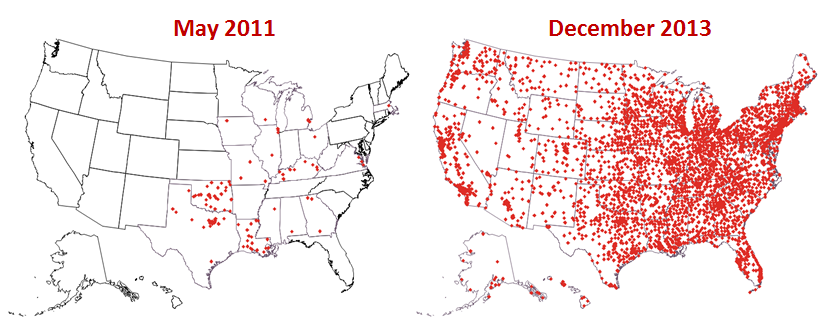
\includegraphics[scale=.5]{graphics/QS-Hospitals-Receiving-Payments-for-MU-and-Adoption.png}
    \caption*{Source: HealthIT.gov}
    \label{fig:meanuse}
\end{figure}

Research on how physicians interact with EHRs is primarily focused on outpatient settings. On a daily basis, a physician spends approximately 23.7\%, 17\%, and 15.5\% of their time on documentation, chart review, and inbox management, respectively, which are the most time consuming portions of EHR use (\cite{arndt2017tethered}). In all, if a physician works for 12 hours, they spend roughly 3.2 hours with patients and 5.9 hours interfacing with an EHR. Despite a large amount of time spent with them, physicians still continue to report frustration over EHR use. The most time consuming functions are also reported as the most frustrating (\cite{dymek2021building}). Another common issue physicians face is the lack of usability of EHR systems, that functions take minutes to either locate or load. Hospitals often provide training upon adoption, but rapid system upgrades and changes make familiarity with the system difficult. While most research is specific to physicians in outpatient settings, the limited research available which investigates hospitalists and EHRs seems to be consistent with these findings (\cite{tipping2010did}). 

\subsection{Hospitalists and Labor Market Decisions}

This section serves to outline the potential responses of hospitalists to EHRs based on their incentives. The behaviors that I consider in this analysis are closely related and should not be taken as independent. For example, hospitalists' choice of work setting depends on their decision to remain in clinical settings, and billing activity depends on work setting. Thus, I discuss the behaviors in stages of decision making. 

For ease of notation, I define a hospitalist in my data as any general practice physician who sees at least 70\% of their patients within a hospital setting. However, there are two types of physicians who can be categorized as hospitalists based on this definition: one being a formal hospitalist, and the other being an internist. Both formal hospitalists and internists are medical professionals who primarily focus on general patient care, but they potentially differ in their work settings. Internists are primary care physicians who provide comprehensive medical care to adult patients in either outpatient settings or hospitals, whereas formal hospitalists specialize in the care of hospitalized patients, and typically work exclusively in the hospital setting. While this distinction is potentially important for some of the decisions outlined below, the data do not explicitely distinguish between the two. I will discuss this limitation in more detail when relevant. 

\subsubsection{Exiting Clinical Work}

There are two main ways for a physician to stop seeing patients altogether: retirement from the labor force in general, or changing careers to non-clinical work. Workers in developed countries tend to plan for formal retirement well in advance. Generally, an exogenous shock to a worker's environment is not expected to change retirement age due to the amount of planning necessary to formally leave the labor force. Classic retirement models structure the decision of retirement by maximizing expected lifetime utility based on future earnings and retirement benefits, or choosing to prolong retirement only if the expected earnings gain from doing so is positive (\cite{gustman1986disaggregated}, \cite{stock1990pension}). However, physicians typically make this decision differently than workers in other industries. Most physicians plan to retire at age 60, but do not actually retire until age 69 (\cite{collier2017challenges}). When the time to retire comes, many physicians hesitate to abandon patients they have seen over the course of their career. The decision to delay retirement is not financial, but altruistic. Thus, retiring may be in a physician's choice set years before the realized decision to leave the labor force. 

Age is the most important factor in the decision to retire, implying that a 35 year old physician has very different incentives than a 65 year old physician, and a technology shock will affect the age groups differently. As a worker considers the retirement decision, they weigh their expected earnings with their expected costs, along with some preferences. Then, a physician will only retire if the utility from working is less than the utility from retiring, where utility partially depends on job satisfaction and personal life factors. Exogenous EHR implementation affects the decision to retire through job satisfaction. If EHRs impose a burden on daily tasks, there is an inverse relationship between EHR exposure and utility from continuing to work. If EHRs make daily tasks easier, there is a positive relationship. Thus, for a physician indifferent between retiring and continuing to work, EHRs induce retirement if they impose a cost in terms of job satisfaction, or induce continued working life if they impose a benefit to job satisfaction. Media articles focusing on interviews with physicians suggest that the implementation of EHRs did in fact lead to retirement in older physicians (\cite{ringel_2019}, \cite{loria_2020}), but this has not been addressed empirically. 

Formal retirement (leaving the labor force altogether) is not the only way for physicians to transition out of a clinical role. There are opportunities for physicians of any age to switch careers towards administrative roles, teaching, consulting, or hospital management. While it is unlikely that early career physicians are formally retiring, physicians of any age could be career switching. This decision is impacted similarly to the above discussion regarding formal retirement, where a physician who is indifferent between clinical work and career switching can be affected one way or the other based on how an EHR impacts job satisfaction. In a 2016 survey, 13\% of physicians stated that they were considering careers outside of clinical work because of burnout (\cite{physicians2016physicians}). As I discuss in Section \ref{sec:data}, I only observe whether a physician stops seeing Medicare patients, not whether they retire or career switch. For the purpose of this paper, the term exit indicates no longer seeing patients, and makes no assertion about what the physician does afterwards.



\subsubsection{Work Setting}

Most physicians are likely not on the margin in their decision to exit clinical work, so EHRs will not impose a large enough cost (or benefit) to impose exit. However, there are other ways hospitalists might change their behavior under drastic changes to their current working environment. For those who remain practicing, changing the physical place of work may allow for more control over which technologies they use. Specifically, if EHRs change job satisfaction of working in the hospital, a hospitalist may decide to shift more of their working hours towards or away from the hospital. Not all physicians working as hospitalists have a binding contract with their associated hospital. In fact, a 2013 survey estimated that 36\% of hospitalists also worked outside of the hospital in primary care, long-term care, or hospice settings (\cite{Today}). Many physicians trained as internists choose to contract their work out to both hospitals and outpatient settings. The fraction of internists who work as hospitalists increased from 25\% to 40\% from 2008 to 2018 (\cite{gray2022evolving}).  

The sample of physicians I consider include both hospitalists with formal contracts and internists who contract a majority of their time with the hospital, but could also work in other settings as well. If a hospital implements a costly EHR, a hospitalist may choose to shift more of their time towards outpatient settings or initiate a contract with outpatient settings to spend less time in the setting where job satisfaction has decreased.


\subsubsection{Productivity}

For those not induced to change their behavior by exiting or changing work settings, it is natural to assess whether EHRs impacted productivity. A main purpose of the HITECH Act was to improve efficiency of care, specifically to decrease time spent on administrative burden. This question is empirically ambiguous since EHRs could add daily tasks that make hospitalists less productive, increase efficiency, or some combination of the two where short term productivity is negatively impacted but long term productivity is positively impacted once physicians adjust and learn the new technology. I measure productivity in terms of the amount of patients a hospitalist is able to see. 

Further, there is a unique relationship between EHR use and efficiency in terms of billing activity done by the hospitalist. Billing activity refers to the number of claims filed per patient seen. There are many reported reasons that physicians tend to over-treat patients, including defensive medicine, patient request, difficulty accessing patient records, and pressure from their institution (\cite{lyu2017overtreatment}). EHRs have the potential to change some of these incentives. As more hospitals adopt EHRs, patient information should be more easily accessible and reduce the amount of repeated tests a physician needs to run, leading to a decrease in claims per patient. However, institutions have power to customize EHRs and train their hospitalists to increase fee-for-service revenue by increasing claims per patient. 





\section{Data}\label{sec:data}

I construct a balanced hospitalist-level panel spanning from 2009-2017 which measures physicians' exposure to EHRs over time, labor market outcomes, and other relevant physician and hospital characteristics. I describe the different data sets used to construct the panel below, and I include a detailed outline of data and variable construction in Appendix \ref{app:data}.

\subsection{Sample Construction}

The Medicare Data on Provider Practice and Specialty (MD-PPAS) is a database of physicians which details claim counts, physician specialty, and practice location from 2009-2017. Variables included are physician NPI, primary and secondary specialties, patient count and total billing counts, and fraction of patients seen in different settings (hospital, office/outpatient, emergency room, etc.). I only include physicians classified as hospitalists\footnote{Physician who self-identifies as hospitalist or has 90\% of patients in inpatient setting. I cannot distinguish between types of hospitalists as the data source manipulates this definition based on percent of patients seen in a hospital, so these can be formal hospitalists or internists.}, internal medicine, general practice or family practice in at least one year. I drop physicians with less than 70\% of patients in a hospital setting in all years, as the focus is on those who are affected by a hospital's decision to adopt (I investigate this threshold in Appendix \ref{sec:changes}). I use this data to construct the dependent variables for my analysis. Generally, these include the decision to exit clinical work, switch to a different work setting, number of patients seen, and billing activity. 


Center for Medicare and Medicaid (CMS) Shared Patient data records annual information on frequency of billing associated with the same patient across providers within a given time period. These data are available from 2009 to 2015. For example, if a primary care physician refers a patient to a specialist, then those two physicians have that particular shared patient in common. The number of shared patients are collected in 30, 90, or 180 day intervals. I focus on the 30 day interval, and I employ this data to detect physicians who work closely with hospitals. I limit the entities by tax-code to only include shared patients for physician-hospital pairs, where the physicians in these pairs match the physicians from MD-PPAS. The types of physicians are already limited to primary care, but there still may be office-based primary care physicians in the shared patient data. Therefore, I limit the sample of pairs based on a threshold of same day patients which depends on the number of years the physician appears in the data. I only include physician-hospital pairs who have non-missing data with at least 30 shared patients per year.


Using hospital National Provider Identifier (NPI), I link the physician-hospital pairs from the Shared Patient data to the American Hospital Association (AHA) survey and the Healthcare Information and Management Systems Society (HIMSS) survey, which both contain information on hospital-level EHR use and other characteristics. I record the first year a hospitalist is exposed to an EHR based on adoption in the hospitals they share patients with. In the AHA survey, a hospital can answer the question of whether they use an EHR with either ``Partially", ``Fully", or ``Not at all". Since partial implementation of an EHR does not guarantee sufficient use, I define a hospital as implementing an EHR the first year they answer ``Fully". In the HIMSS data, hospitals report the specific vendor they employ. From this, I define the first year a hospital reports using a vendor. I combine these measures to define the first year a hospital reports using an EHR in either survey. While there is an AHA survey supplement which captures more granular details about information technology, only a small subset of hospitals choose to answer this survey. In this paper, I focus on the initial shock of any new technology and abstract away from some of the more granular characteristics of the technology.

I aggregate the data to the physician level. I drop physicians who are not treated by 2015 since I do not observe whether they become treated in 2016 or 2017.\footnote{In Appendix \ref{sec:changes} I limit years to 2009-2015 and include never-treated. The results are robust to this specification choice.} That is, the data contains no units which are ``never-treated". Finally, I include a physician's graduation year from Physician Compare (provided by CMS). I limit to physicians who graduated before 2005, as anyone who graduated medical school after that will be finishing residency during the span of the data and will exhibit labor market changing behavior which could be correlated to EHR exposure purely because of switching work settings during a time of rapid EHR implementation.There are various thresholds used in the construction of this final data, including how many shared patients constitutes a physician-hospital relationship. The details of such thresholds are explained in Appendix \ref{app:data}. To ensure that my results  are not sensitive to various levels of the thresholds, I estimate the effect of EHR exposure on all outcomes under different combinations of data limitations. The specification charts with these results are shown in Appendix \ref{sec:chart}, and I discuss each in conjunction with the main results. 

The first dependent variable I consider is the decision for a physician to stop seeing Medicare patients, which I refer to as exit. Exit is an indicator variable equal to 1 in the first year that a hospitalist sees no patients in any future year and zero in every other year. This captures a one time decision to stop seeing patients, not a cumulative decision in all following years. The next variables I construct capture whether physicians change work setting. I consider the fraction of patients a physician sees in an office-based/outpatient setting, and I construct an indicator variable equal to one if a physician sees any positive number of patients in such a setting. Finally, I consider outcome variables which explore productivity and efficiency, the number of patients seen and claims filed per patient.


\subsection{Summary Statistics}

For each progression of decision making, I limit to physicians who did not change their behavior previously. That is, for office-based outcomes I exclude physicians who exit, and for productivity outcomes I exclude physicians who exit or change their work setting. I show summary statistics of relevant variables based on each sample in Table \ref{tab:sumstats}. 

\import{Table Code}{overall stats.tex}

\normalsize
I follow a maximum of 19,263 hospitalists over time, depending on the sample considered. Out of all hospitalists in the sample, 3\% (approximately 578) stop seeing patients at some point. A positive number of hospitalists are exposed to an EHR in each year, but the majority of exposure is concentrated towards early years. For hospitalists in the office setting sample (those who do not exit), 30\% of physicians have a positive number of patients seen in an office, and the average physician sees 9\% of their total patient volume in an office. There are 12,732 hospitalists who never exit or change their work setting at any point in the sample. These hospitalists see 325 patients and file 4 claims per patient on average. Consistent across all samples, hospitalists tend to work with 1.3 hospitals and 1.2 systems. 


In Figure \ref{fig:treatmentgraph}, I present a graph of the variation in treatment over time and the underlying hospital adoption that drives this treatment variable. Hospitalists are exposed the first time one of their hospital's adopts an EHR. Thus, I show the percent of hospitals adopting as well as the percent of hospitalists exposed to the technology. In 2009, 41\% of all hospitalists were already exposed to an EHR. That is, half of the sample had no affiliation with EHRs at the beginning of the sample period. Since I drop any physicians who do not have exposure to an EHR by 2015, 100\% of the sample is exposed by the end of the sample period. In 2009, 47\% of hospitals have adopted an EHR, and this percentage grows steadily over time, driving the increase in exposed hospitalists. 

\begin{figure}[t]
\centering
\captionsetup{width=.45\linewidth}
    \caption{Treatment Variables Over Time}
    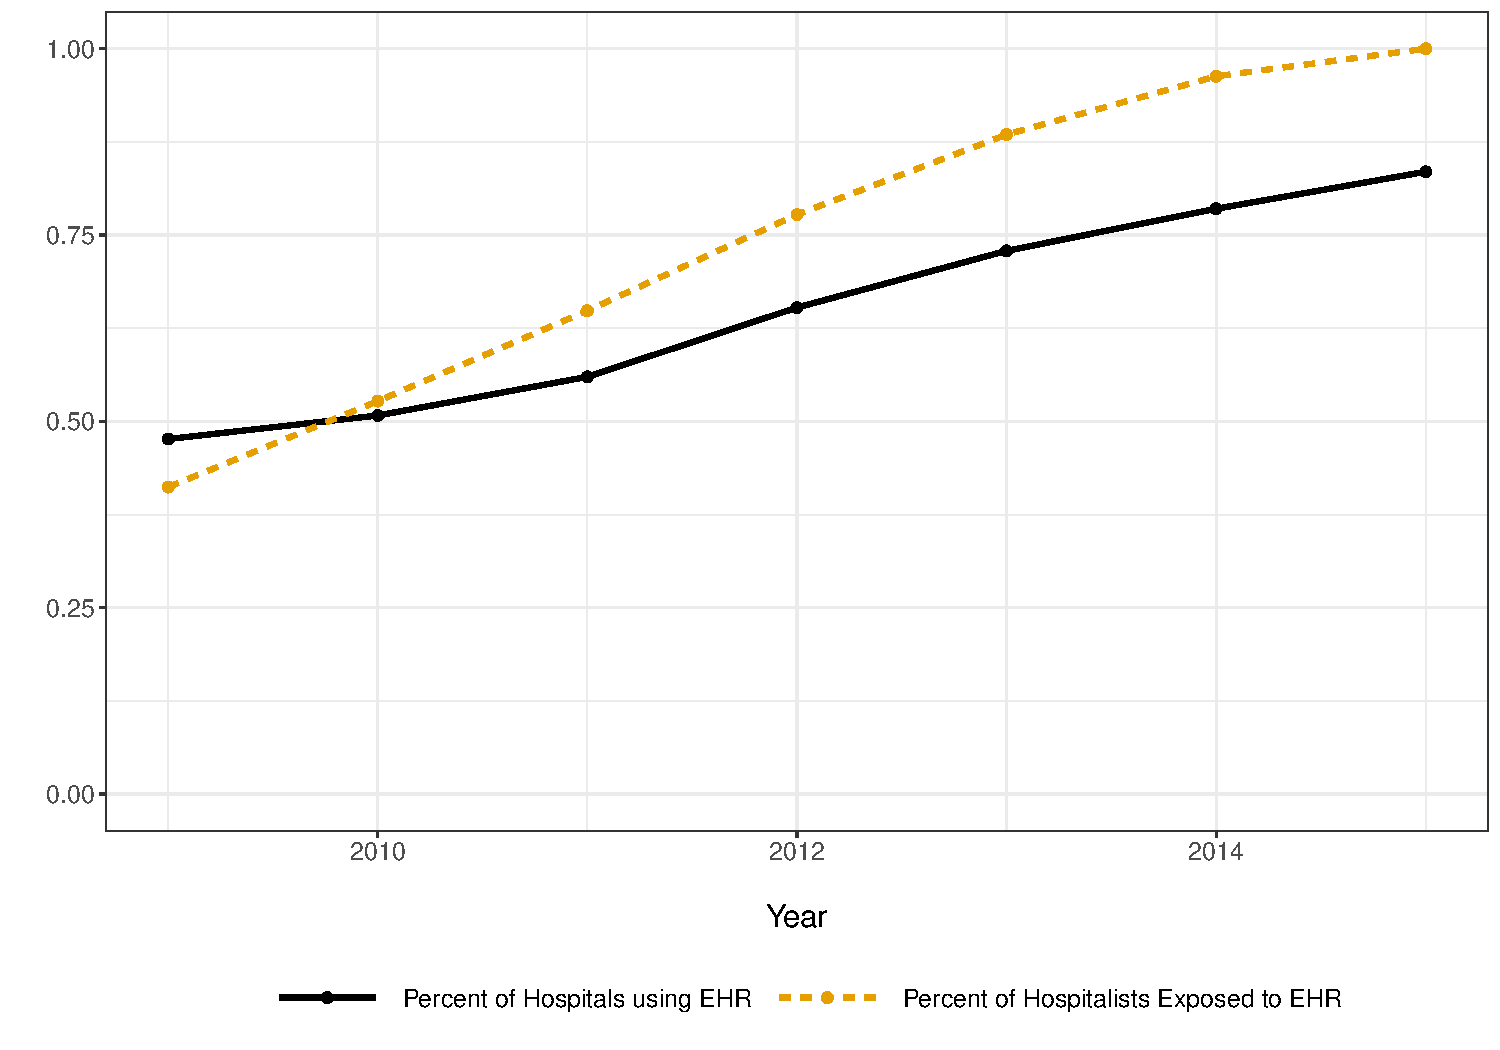
\includegraphics[scale=.6]{Objects/sum_stats_year.pdf}
    \label{fig:treatmentgraph}
\end{figure}



\section{Empirical Strategy}\label{sec:empstrat}

I estimate average treatment effects of EHR exposure on the outcomes discussed. In this setting, treatment effects may be heterogeneous across hospitalists who are exposed in different years since the underlying characteristics of hospitals who adopt in different years may be correlated with the decision to adopt. Therefore, to avoid negative weighting issues this causes in a classical two way fixed effects event study specification, I instead estimate average treatment effects for a specific group $g$ at time $t$: 
$$ATT(g,t)=\mathbbm{E}[Y_t(g)-Y_t(0)|G_g=1],$$
where $G_g=1$ for those in group $g$. A group indicates all hospitalists treated, or first exposed to an EHR, in the same year. I employ the doubly robust estimator established in \citeauthor{sant2020doubly} (\citeyear{sant2020doubly}). Other estimators that similarly address the concerns yield similar results, presented in Appendix \ref{app:estimators}. I also present classical two way fixed effects results with physician and year fixed effects in Appendix \ref{app:estimators}.

I aggregate the group time estimates over groups to a more familiar event study plot with simultaneous confidence bands calculated using bootstrapped standard errors. Further, a weighted average of estimates is taken to provide a single $ATT$ value for each outcome; these values are presented in the notes of each results plot. 

\subsection{Identification Assumptions}

There are several assumptions necessary to identify the parameters of interest, $ATT(g,t)$. First, I assume that treatment is not reversed. That is, once a hospitalist is exposed to an EHR, they cannot be un-exposed. For hospitalists that do not switch hospitals, this assumption is supported by the institutional details of hospital EHR implementation. An EHR is a costly technology and requires a significant amount of collaboration to implement, so a hospital does not have incentive to un-implement an EHR. They may add features or switch vendors, but do not reverse EHR use. Any hospitalists included in the productivity sample are those which did not switch work settings, satisfying this assumption.

Second, I assume hospitalists do not anticipate EHR exposure prior to occurrence. If they learn that the system will be implemented and change their behavior beforehand, the estimates may be biased. Generally, even a complex EHR system can be completely set up within a year, and most systems take 6 to 9 months (\cite{uzialko_2021}). Therefore, I proceed in the main specification assuming no anticipation. However, I explore and present results for a one year anticipation period in the specification charts in Appendix \ref{sec:changes}, and I find that accounting for one year of anticipation does not drastically change the findings.  

As is usual in a difference-in-differences framework, I assume a version of parallel trends based on not-yet-treated units. I assume that, conditional on years of experience, average outcomes for those treated in group $g$ would have followed a parallel trend as those in groups treated in later periods. While this assumption cannot be tested directly, I present p-values for a Wald test of pre-trends. Further, I investigate pre-trends extensively in Appendix \ref{sec:pretrends} by allowing for specified violations in the parallel trends assumption (\cite{rambachan2019honest}). I find that most outcomes are very robust to violations in the parallel trends assumption. 

To interpret these estimators as the causal effect of EHR exposure on various labor market outcomes, there are additional institutional assumptions necessary. First, I assume that when a hospitalist works in an electronic record utilizing-hospital, they utilize the electronic health record system fully. That is, the hospitalist does not continue practicing without using the EHR. While some hospitalists may create work-arounds to ease the burden of EHR use, it is inevitable that they will need to interact with the technology in some capacity. Second, I assume that a physician's exposure to EHRs is exogenous. That is, the physician does not influence the hospital's decision to implement an EHR.


\section{Effect of EHR Exposure on Labor Market Outcomes}


\subsection{No Longer Seeing Patients}\label{sec:retire}


I present aggregated group time treatment effects of being exposed to an EHR on the likelihood of exiting clinical work for the full sample of hospitalists, as well as split samples for those at least 60 (typical retirement age) and less than 60 years of age in Figure \ref{fig:retirefirst}.\footnote{Alternatively, one could estimate the effect for more age groups and observe the relationship between the overall ATT and age. However, the data does not support further sub-setting as sample sizes become small.} These effects are a weighted average of the $ATT(g,t)$ parameters discussed in Section \ref{sec:empstrat}. Being exposed to an EHR leads to a .2 ppt increase in the likelihood of exiting in the first year after exposure, and a .4 ppt increase in the second year after exposure. While numerically small, these effects are economically meaningful relative to the proportion of hospitalists who exit in the sample, .03. That is, the effect represents a 7\% (13\% in the second year) increase in the likelihood of exiting relative to the mean.   

\begin{figure}[ht!]
\centering
    \captionsetup{width=.85\linewidth}
    \caption{Effect of EHR Exposure on Retirement}
   \begin{subfigure}[]{.8\textwidth}
   \caption{all physicians}
   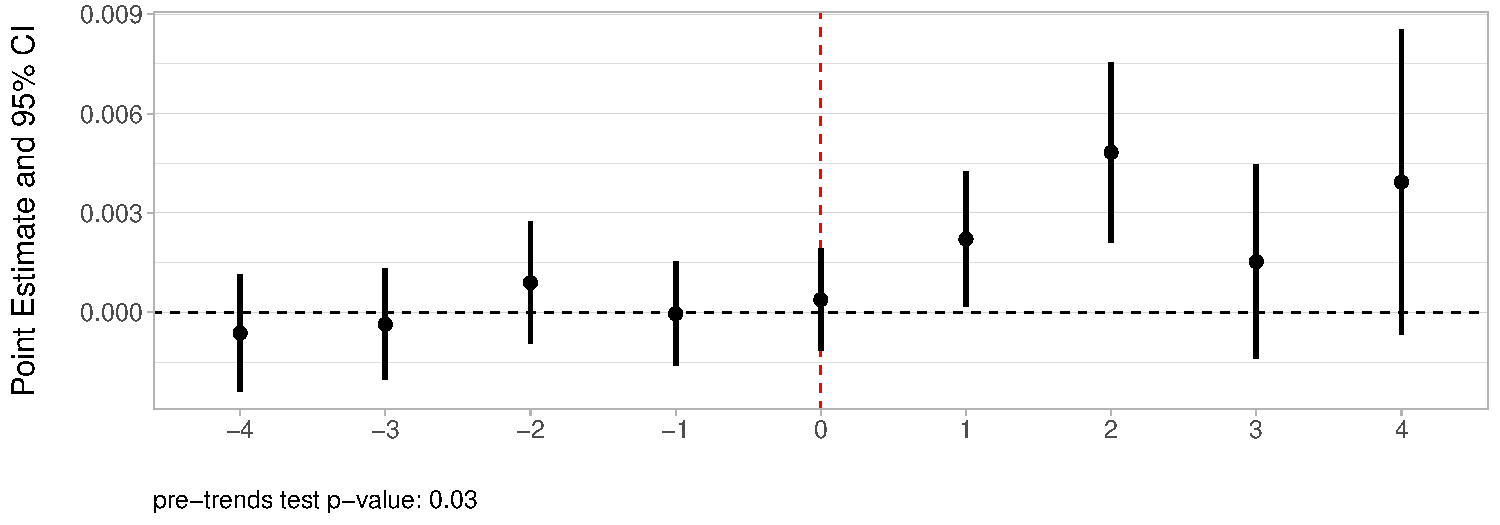
\includegraphics[scale=.55]{Objects/retire_plot_all.pdf}
   \label{fig:retirefirst} 
\end{subfigure}

\vspace{1.5mm}

\begin{subfigure}[]{.8\textwidth}
\caption{sub-samples of physicians based on age}
   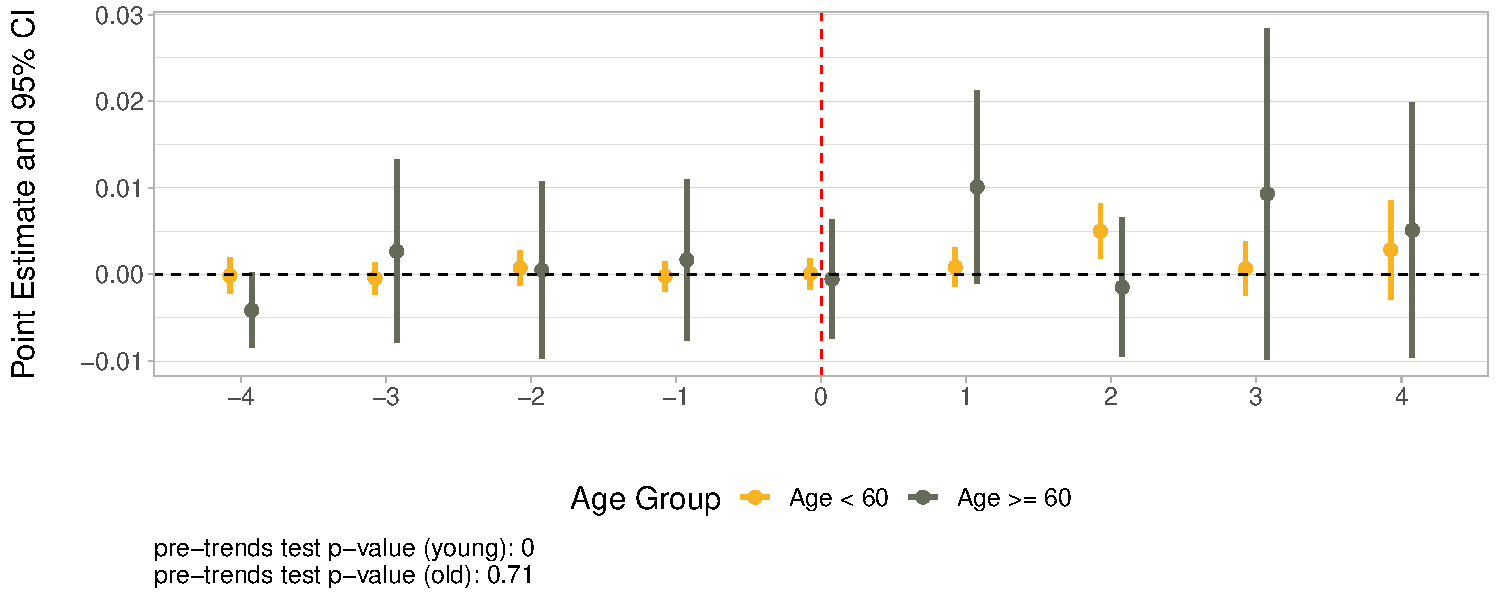
\includegraphics[scale=.55]{Objects/retire_plot_ages.pdf}
   \label{fig:retiresecond}
\end{subfigure}
\vspace{2mm}
    \caption*{\footnotesize{\textit{Notes:} Panel (a) shows average group time treatment effects aggregated over groups to an event study plot. Panel (b) shows these results for different subgroups of physicians by age. The p-value listed for each graph corresponds to a Wald test for pre-trends. Confidence intervals shown are simultaneous confidence bands accounting for multiple hypothesis testing. ATT for all, $<$ 60, $>=$ 60 with SE in parentheses: 0.003 (0.0009), 0.002 (0.001), 0.006 (0.003), respectively.}}
\end{figure}


Next, I examine how the results differ when considering physicians in different age brackets: pre-retirement ($<= 60$) and typical retirement age ($> 60$). Interestingly, hospitalists >=60 are driving the positive estimate in the year after exposure, and younger hospitalists only exit in the second year after exposure. A retirement age physician is 1 ppt more likely to exit after being exposed to an EHR, a 25\% increase relative to the mean. In comparison, hospitalists less than 60 are not more likely to exit in the first year after exposure, but are approximately 16\% more likely to exit two years after exposure. There are two potential reasons for the different response time that relate to formal retirement vs. career switching. First, if younger physicians are leaving clinical work for administrative or consulting roles, the preparation time for this type of switch (preparing a resume, applying for new jobs, etc.) could be longer than one year, whereas formal retirement can be decided and executed within one year. Similarly, younger hospitalists may attempt to learn complex EHRs for a longer period of time before deciding the cost is too high. 

There is no visual indication of a violation of the parallel trends assumption in the pre-periods. However, the p-value of a Wald test for pre-trends indicates some evidence for such a violation for younger hospitalists. In Appendix \ref{sec:pretrends}, I present confidence intervals robust to various specifications of a violation in parallel trends. Due to the rarity of exiting for this sub-sample, the estimate becomes null with any specified variation in the parallel trend assumption. I still discuss the estimates for this age group, but focus on the results for the older hospitalists. I also present overall treatment effects under different data specifications in Appendix \ref{sec:chart}, and find that this result is robust to various specifications. 

A potential concern is that hospitalists are not leaving a clinical setting, but choosing to only see patients with private insurance. First, EHR use should not be directly correlated with Medicare patients. Further, as a hospitalist, these physicians do not have complete control over their patient composition and are not paid differently based on the types of patients they see. As a final check, the CMS publishes a list of physicians who have officially opted out of seeing Medicare patients and none of the hospitalists in the sample have selected into this option. 


\subsection{Work Setting}

I investigate another dimension by which hospitalists could change behavior: the extent to which they work in an office (outpatient setting) and whether this changes due to EHR exposure. The outcomes I consider are (1) an indicator variable equal to 1 if the hospitalist has any positive number of patients in an office in a given year, shown in Figure \ref{fig:officefirsta}, and (2) the fraction of patients a hospitalist sees in an office in a given year, shown in Figure \ref{fig:officeseconda}. This analysis does not include individuals who exit at any point in the sample, as a zero could indicate dropping out of the data instead of working solely in a hospital. 

EHR exposure increases the likelihood of working in an office by at least 4 ppts in every year after being exposed, where the effect increases over time (up to 10 ppts four years after exposure). This estimate is equivalent to a 15-38\% increase relative to the average proportion of hospitalists who work in an office. That is, those working only in a hospital are more likely to start working in an office after being exposed to an EHR, and these effects are just as large as those on exiting. However, unlike the estimated exiting effects, the increased likelihood of working in an office is persistent over time, which suggests that EHRs impact work environment in hospitals for several years after implementation. 

\begin{figure}[ht!]
\centering
    \captionsetup{width=.85\linewidth}
    \caption{Effect of EHR Exposure on Likelihood of Working in Office}
   \begin{subfigure}[]{.8\textwidth}
   \caption{all physicians}
   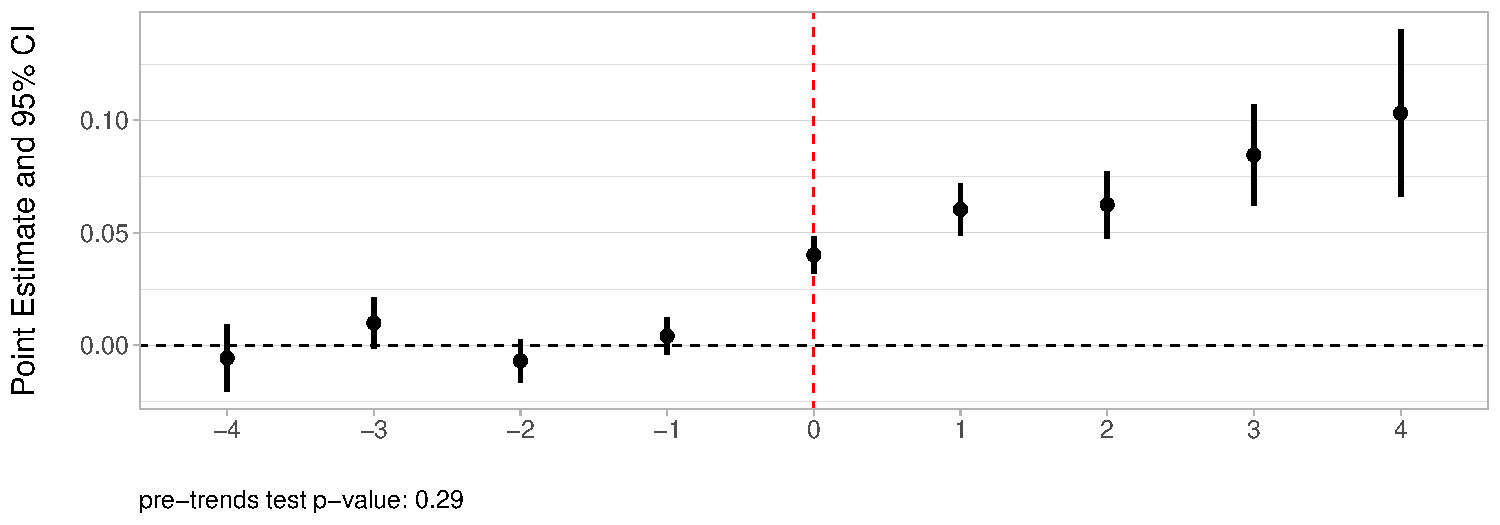
\includegraphics[scale=.55]{Objects/officeind_plot_all.pdf}
   \label{fig:officefirsta} 
\end{subfigure}

\vspace{3mm}

\begin{subfigure}[]{.8\textwidth}
\caption{sub-samples of physicians based on age}
   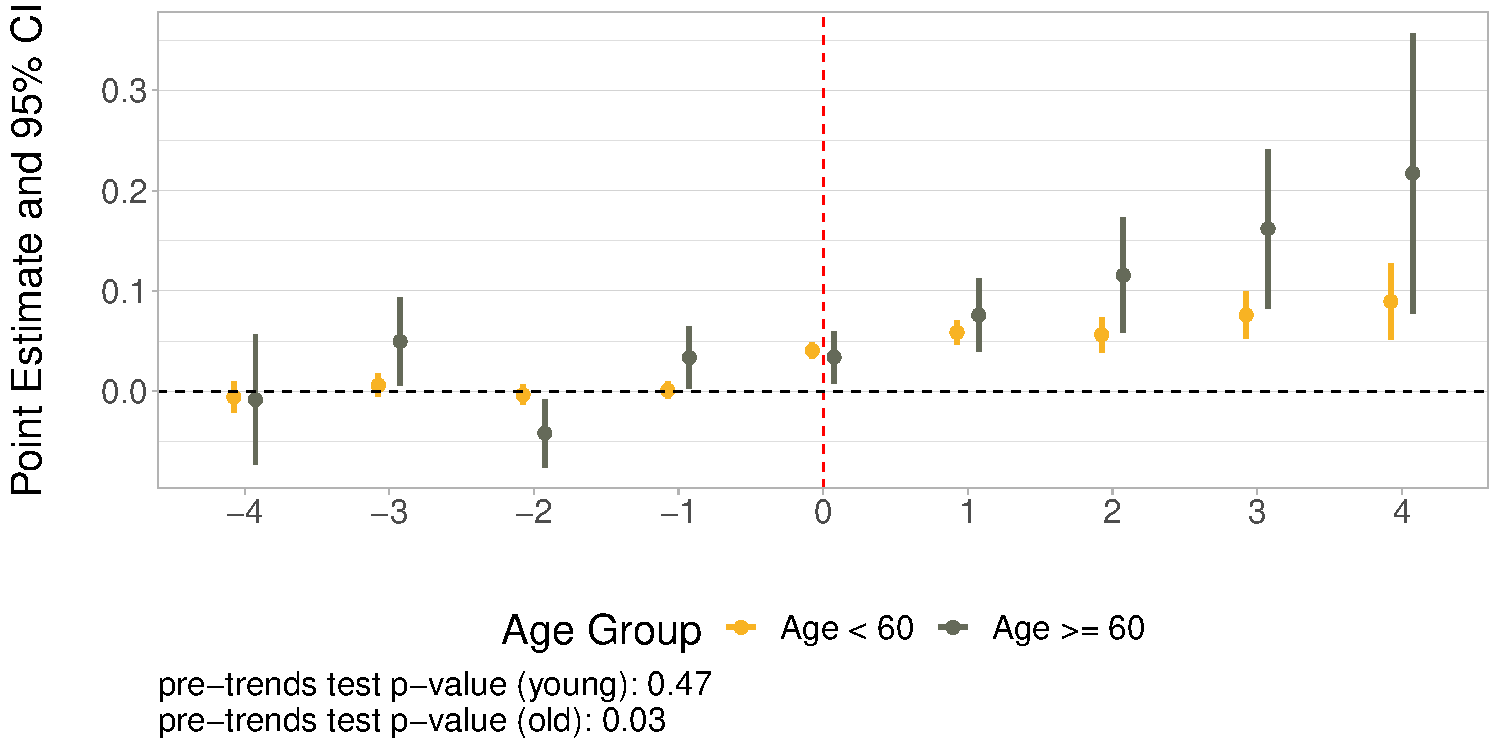
\includegraphics[scale=.55]{Objects/officeind_plot_ages.pdf}
   \label{fig:officefirstb}
\end{subfigure}
\vspace{2mm}
    \caption*{\footnotesize{\textit{Notes:} The top panel shows average group time treatment effects aggregated over groups to an event study plot. The bottom show these results for different subgroups of physicians by age. The p-value listed for each graph corresponds to a Wald test for pre-trends. Confidence intervals shown are simultaneous confidence bands accounting for multiple hypothesis testing. Overall ATT for all, $<$ 60, $>=$ 60 with SE in parentheses: .07 (0.008), .06 (0.008), 0.12 (0.03), respectively}}
\end{figure}


To continue investigating how different ages may respond differently to technology, I also present estimates for hospitalists less than 60 and greater than or equal to 60 separately in Figure \ref{fig:officefirstb}. Unlike the choice to exit, the age groups are both responding to EHR implementation in all years after exposure. The magnitudes for senior hospitalists continue to increase over time, whereas the estimates for younger physicians level out. However, senior physicians are more likely to work in an office than younger physicians on average, so both groups exhibit similar increases relative to the mean. 

The previous results are driven by hospitalists who are not working in an office prior to EHR exposure, but it could also be the case that hospitalists who already work in both settings before exposure change the amount of work they do in an office. Thus, I estimate the effect of EHR exposure on the fraction of patients seen in office based settings.\footnote{Since this variable is tied to the total number of patients seen, I also estimate this analysis with the outcome of total number of patients seen in an office and the results are identical.} The estimates, displayed in Figure \ref{fig:officeseconda}, show an increase in the fraction of patients seen in office settings after the hospitalist is exposed to an EHR. In the year of exposure, the fraction of patients increases by .04, and by the fourth year after exposure the fraction of patients increases by .12. Since the hospitalists included in the sample are meant to have close ties with hospitals, the average fraction of patients seen in an office is low, at .09. Thus, the observed effect is massive, as it is equivalent to a 75-150\% increase in the fraction of patients seen in an office relative to the mean. Further, the variation in this variable can either be driven by physicians who already worked in an office or those who did not and then began working in an office after exposure. When I partition the sample into prior office work, the effects are identical for both groups. 


\begin{figure}[ht!]
\centering
    \captionsetup{width=.85\linewidth}
    \caption{Effect of EHR Exposure on Fraction of Patients Seen in Office}
   \begin{subfigure}[]{.8\textwidth}
   \caption{all physicians}
   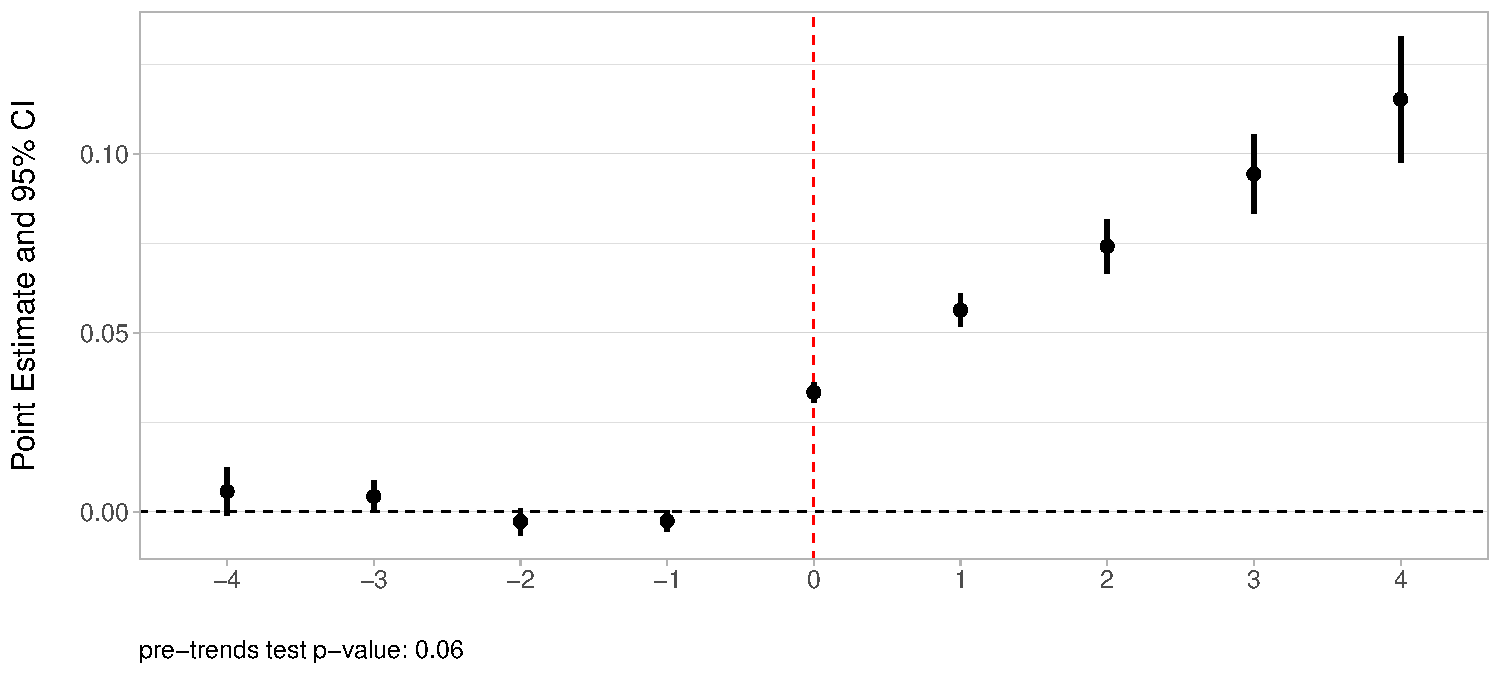
\includegraphics[scale=.55]{Objects/officefrac_plot_all.pdf}
   \label{fig:officeseconda} 
\end{subfigure}

\vspace{3mm}

\begin{subfigure}[]{.8\textwidth}
\caption{sub-samples of physicians based on age}
   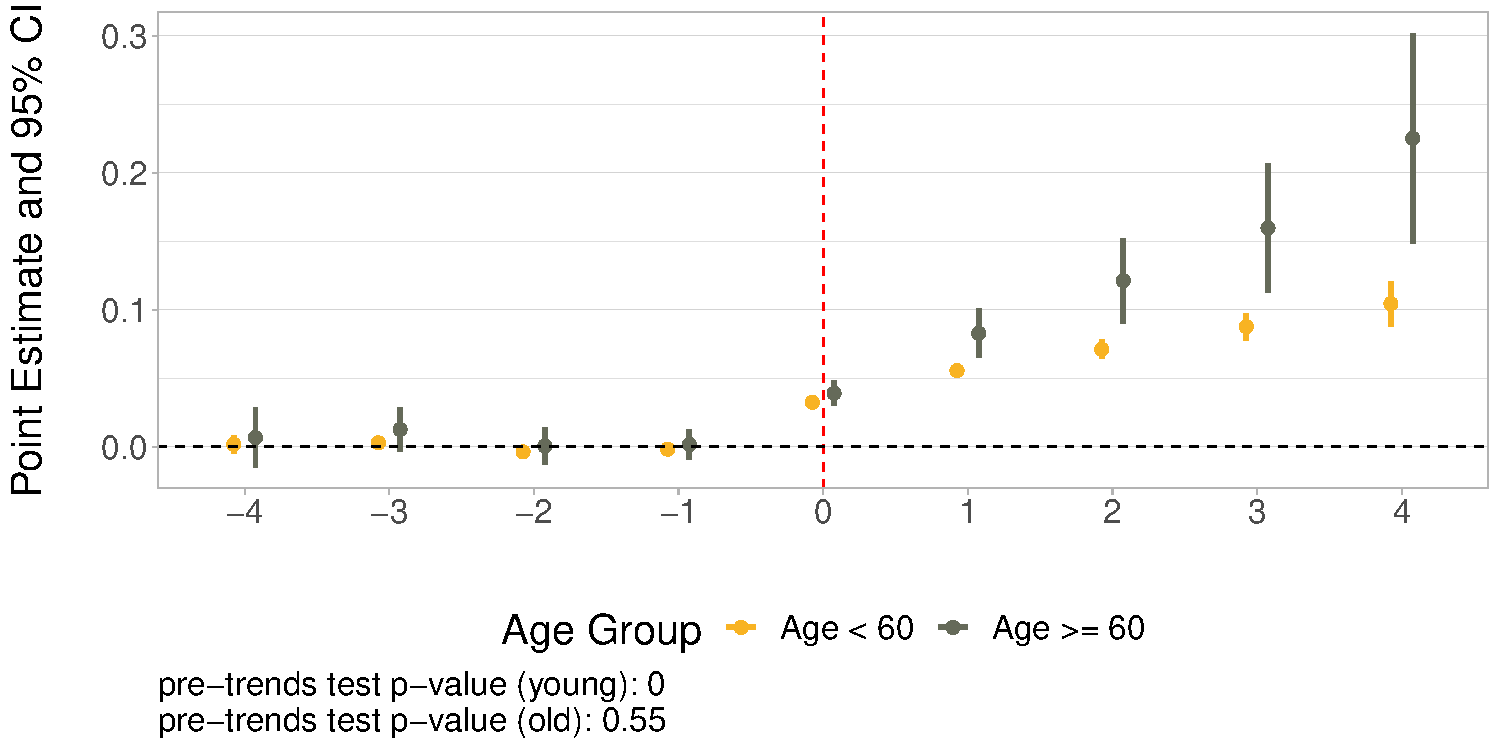
\includegraphics[scale=.55]{Objects/officefrac_plot_ages.pdf}
   \label{fig:officesecondb}
\end{subfigure}
\vspace{2mm}
    \caption*{\footnotesize{\textit{Notes:} The top panel shows average group time treatment effects aggregated over groups to an event study plot. The bottom show these results for different subgroups of physicians by age. The p-value listed for each graph corresponds to a Wald test for pre-trends. Confidence intervals shown are simultaneous confidence bands accounting for multiple hypothesis testing. Overall ATT for all, $<$ 60, $>=$ 60 with SE in parentheses: .08 (0.003), .07 (0.003), 0.13 (0.01), respectively.}}
\end{figure}


I also investigate pre-trends for these outcomes in Appendix \ref{sec:pretrends}, where I find that under various assumptions of the form of violation in parallel trends, the estimate remains positive and significant of similar magnitude. Further, under different combinations of data specifications I find consistently positive and significant results, as shown in Appendix \ref{sec:changes}. 


\subsection{Patient Count and Billing Activity}\label{sec:patientcount}

As a measure of productivity/efficiency, I now estimate the effect of EHR exposure on patient count and billing activity per patient. I limit to hospitalists who work with the same one hospital through the entire sample. These hospitalists do not exit or see patients in another hospital, so that when an EHR is implemented the they remain utilizing the EHR for the remainder of the sample. The effect of EHR exposure on patient count is shown in Figure \ref{fig:patienta}. For hospitalists of any age, patient count increases by 22 patients in the year of EHR exposure, 55 patients in the year after exposure, 40 patients in the second year after exposure, 30 and 20 patients in the third and fourth year after exposure. These estimates translate to a 6-17\% increase in the number of patients seen relative to the mean. Interestingly, when splitting the sample by age group, the effect decreases three and four years after exposure for younger hospitalists, while the effect for senior age hospitalists remains persistent over time, suggesting that technology's effect on productivity in the long run depends on worker type (in this case, age). 

\begin{figure}[ht!]
\centering
    \captionsetup{width=.85\linewidth}
    \caption{Effect of EHR Exposure on Number of Patients Seen}
   \begin{subfigure}[]{.8\textwidth}
   \caption{all physicians}
   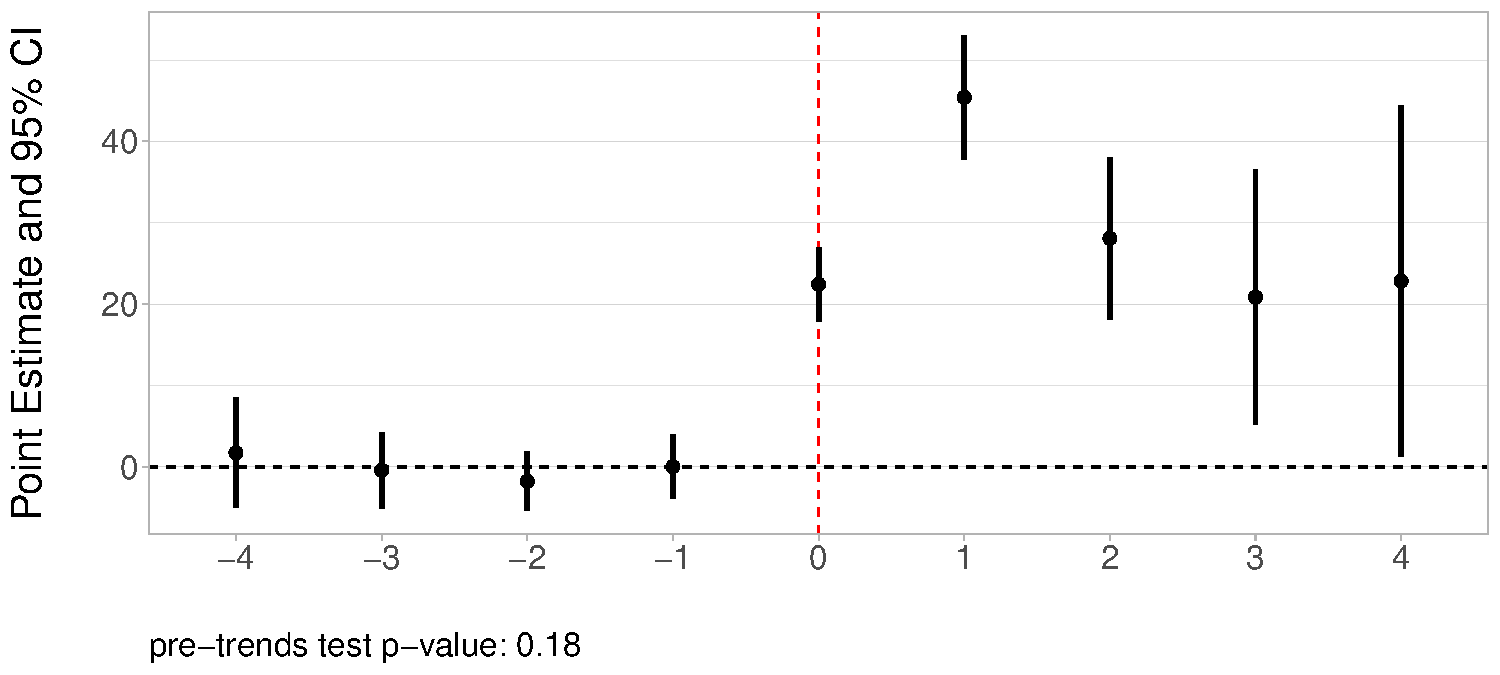
\includegraphics[scale=.55]{Objects/patient_plot_all.pdf}
   \label{fig:patienta} 
\end{subfigure}

\vspace{3mm}

\begin{subfigure}[]{.8\textwidth}
\caption{sub-samples of physicians based on age}
   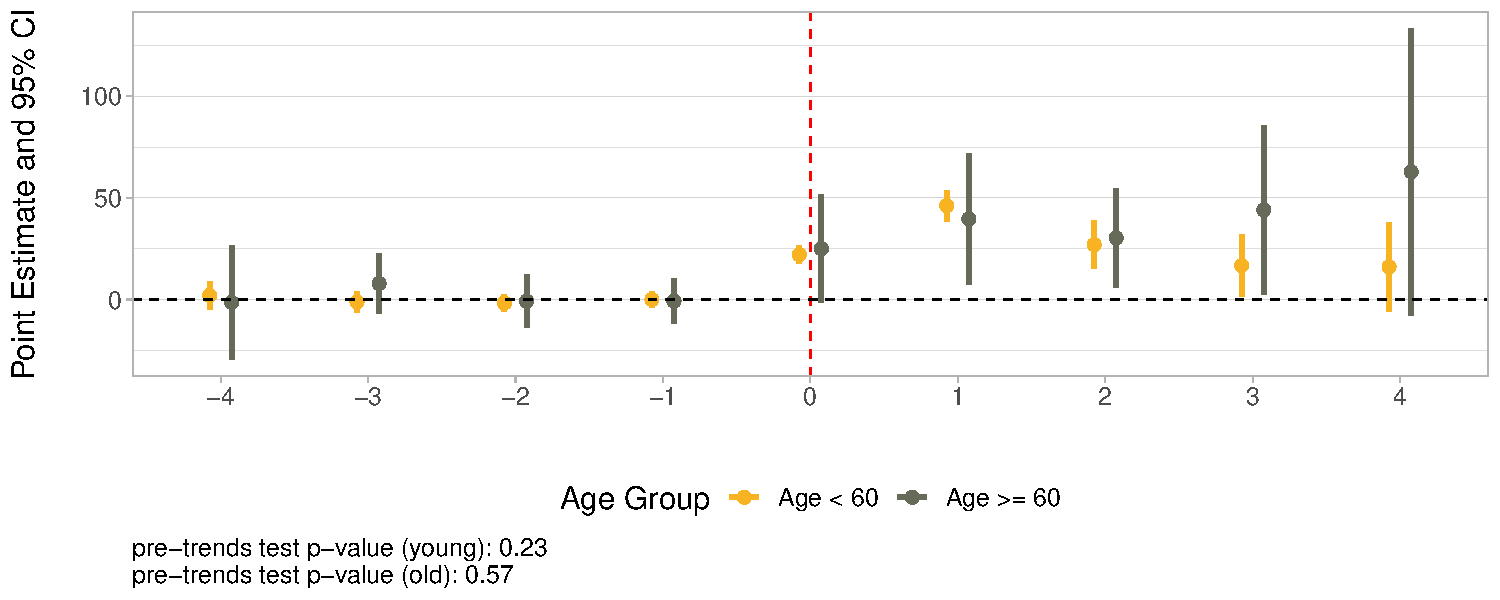
\includegraphics[scale=.55]{Objects/patient_plot_ages.pdf}
   \label{fig:patientb}
\end{subfigure}
\vspace{2mm}
    \caption*{\footnotesize{\textit{Notes:} The top panel shows average group time treatment effects aggregated over groups to an event study plot. The bottom show these results for different subgroups of physicians by age. The p-value listed for each graph corresponds to a Wald test for pre-trends. Confidence intervals shown are simultaneous confidence bands accounting for multiple hypothesis testing. Overall ATT for all, $<$ 60, $>=$ 60 with SE in parentheses: 28 (5.0), 25.6 (5.2), 40.4 (15.0), respectively.}}
\end{figure}

While I am investigating the supply side factors of this outcome, patient count is also driven by demand for health care. A major change in the U.S. health care system, the Affordable Care Act (ACA) was passed in 2010 and took effect in 2014. If my results are driven primarily by the group of hospitals who implemented EHRs in 2014, one might be concerned that the legislation may be driving the increased patient count. The ACA had potentially opposing effects on Medicare patients: they may be crowded out by an increased demand in Medicaid patients, or the small changes to Medicare may have led to an increase in utilization from the Medicare population. A recent study found no negative spillovers to the Medicare population due to the ACA (\cite{carey2020impact}), suggesting that demand change should not drive my results. Additionally, I present average group time treatment effects for each treated group in Figure \ref{fig:patientgroup} of the appendix. Each group shows the same pattern of an increase in patient count after exposure, suggesting that the groups affected by the ACA are not driving the results. 

EHR exposure affects which hospitalists are included in this analysis (since I drop those who exit or move), indicating a non-random attrition problem. That is, if productive or tech savvy hospitalists are the ones who remain in the same hospital after EHR exposure, the estimates are biased. The proportion of those who are not included in this analysis is 18\% in the control group and 36\% in the treated group. To investigate whether my results are robust to this issue, I construct average treatment effect bounds as in  \citeauthor{lee2009training} (\citeyear{lee2009training}). For these bounds to be valid, a monotonicity assumption must hold on selection. That is, treatment can only affect selection in one direction. In my case, that means that EHR exposure increases the likelihood of exiting or moving workplace settings and no hospitalists remain in the sample under treatment who would have exited or moved in the absence of EHR exposure. Since I find in earlier analyses that hospitalists are more likely to move and exit due to EHRs, this assumption is reasonable. To compute the bounds, I trim the distribution of patient count in the control group by the difference in attrition rate. Trimming the bottom (top) and taking the differences in expectation between treatment and trimmed control provides a lower (upper) bound. This bounding yields an interval estimate of 54.6 patients to 125.4 patients, compared to the main result of 28 patients. The bound therefore suggests selection of physicians pushes the estimate down.

Similarly, I investigate whether this increase in the number of patients seen is due to the decrease in the number of working hospitalists. Specifically, a hospital that loses a portion of their physicians, and divides those patients among those remaining. In the long run, the hospital should hire new hospitalists to replace those that left, but in the short run estimates could be driven by increased workload instead of EHR use. This could explain why there is a much larger increase in the first year after exposure compared to the magnitudes of the estimates as they level out over time. Using the estimates I found in Section \ref{sec:retire}, I calculate the increase in the number of patients that would occur if all patients from hospitalists who exited were divided between remaining hospitalists. In the year of exposure the entire increase in patient count is due to EHR use since I find no effect on the likelihood of exit. In the first year after exposure, I estimate the increase in patients due to exiting physicians to be approximately 20 patients, which is less than the observed patient count estimates presented above. However, the second year after exposure is when I observe that largest effect on exiting, and so I do not rule out that the increase in patient count for every year after the first could be caused by the decrease in hospitalists. 

Finally, I consider whether EHR exposure affects claims filed per patient. On average, hospitalists file roughly 4 claims per patient. I present estimates in Figure \ref{fig:claima}, which shows that EHRs tend to increase claims filed per patient over time. The magnitude of the effect ranges from .2 to .8, or 5-20\% relative to the mean, indicating that as hospitalists are exposed to the new software, they bill for more items on average.  I also show heterogeneity of this result by age group, and Figure \ref{fig:claimb} shows that younger hospitalists are exhibiting more of an increase in claim count than older hospitalists.

There is no evidence of a pre-trend driving this result, and I also show robustness to violations in parallel trends in Appendix \ref{sec:pretrends}. I also compute \citeauthor{lee2009training} (\citeyear{lee2009training}) bounds for this outcome due to the limited sample. The computed bounds on the average treatment effect are .45 to .6 claims per patient, compared to the overall effect in the main specification of .33. The effect becomes even larger when accounting for a particular type of physician being left in the sample. However, when I analyze this relationship under different data specifications (shown in Appendix \ref{sec:chart}, around half of the estimates are null. Anticipation and limiting sample years cause the effect to disappear or even become negative. Thus, it is not clear whether this positive effect is actually an unintended consequence of EHRs. 
     

\begin{figure}[ht!]
\centering
    \captionsetup{width=.85\linewidth}
    \caption{Effect of EHR Exposure on Claims per Patient}
   \begin{subfigure}[]{.8\textwidth}
   \caption{all physicians}
   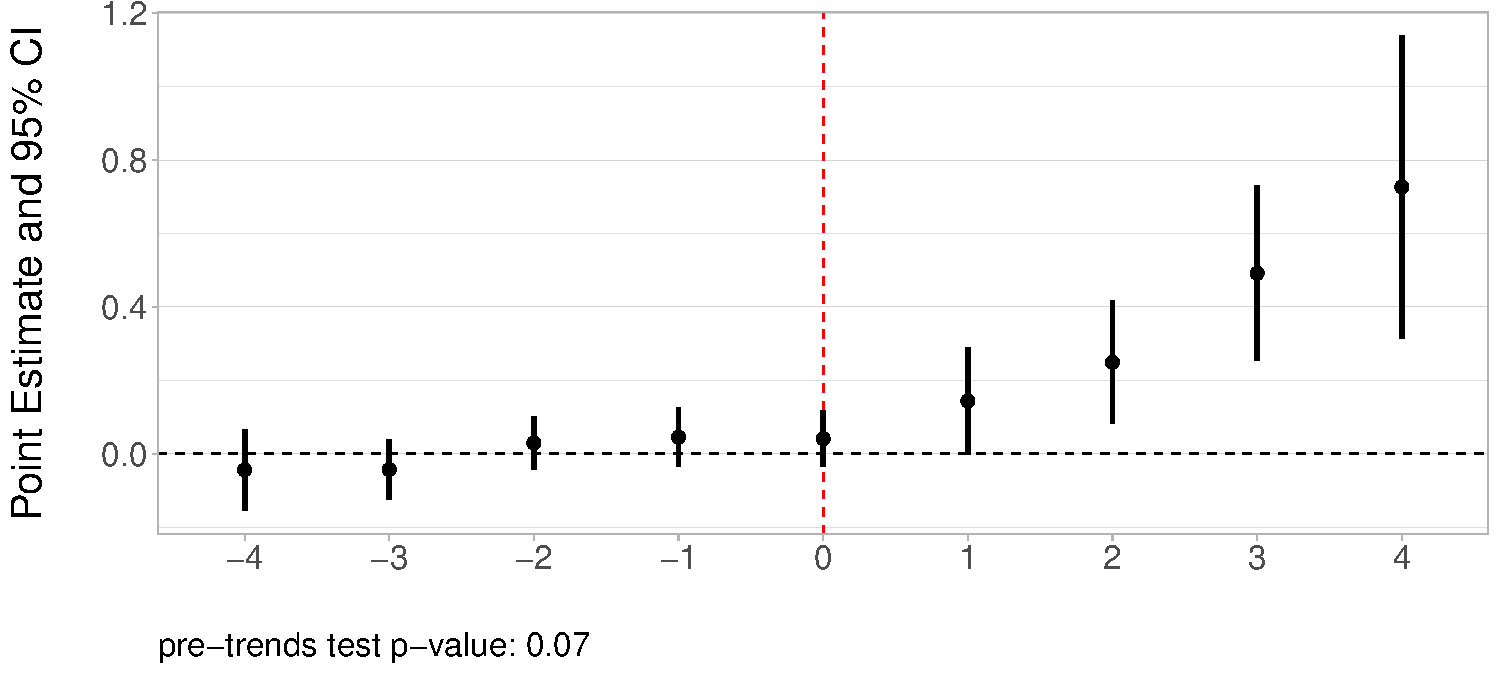
\includegraphics[scale=.55]{Objects/claim_per_patient_plot_all.pdf}
   \label{fig:claima} 
\end{subfigure}

\vspace{3mm}

\begin{subfigure}[]{.8\textwidth}
\caption{sub-samples of physicians based on age}
   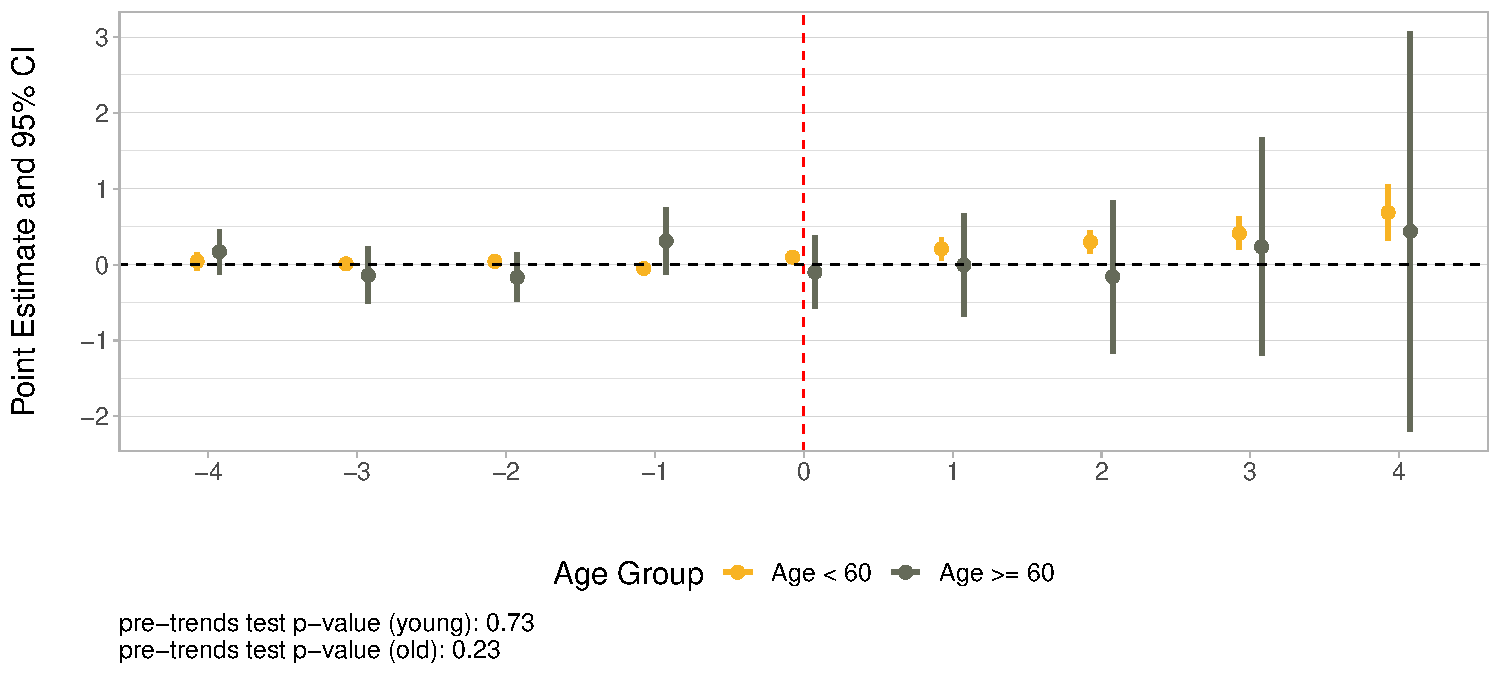
\includegraphics[scale=.55]{Objects/claim_per_patient_plot_ages.pdf}
   \label{fig:claimb}
\end{subfigure}
\vspace{2mm}
    \caption*{\footnotesize{\textit{Notes:} The top panel shows average group time treatment effects aggregated over groups to an event study plot. The bottom show these results for different subgroups of physicians by age. The p-value listed for each graph corresponds to a Wald test for pre-trends. Confidence intervals shown are simultaneous confidence bands accounting for multiple hypothesis testing. Overall ATT for all, $<$ 60, $>=$ 60 with SE in parentheses: .33 (.09), .37 (.08), .05 (.44), respectively.}}
\end{figure}


\section{Conclusion}

A technology expected to revolutionize the health care system was the advancement of health information technology in the form of complex electronic health record (EHR) systems. While they have the potential to improve efficiency, cut costs, and increase quality of care, these results have not come to fruition as expected. While the effect of EHRs on these outcomes has been directly studied, there is a gap in understanding how physicians, the primary user of this technology, responded to their rapid implementation of EHRs. In this study, I analyze the effect of implementing electronic health records on various labor market choices of hospitalists, since EHRs have been controversial and speculated as a cause of burnout. Understanding how hospitalists respond to this technology is important, as physician labor markets have implications for access to care, quality of care, and costs. 

I utilize data on shared patients between medical entities, hospital EHR use, and physician billing activity to analyze this relationship. Using a difference-in-differences framework, I find that hospitalists are more likely to leave clinical settings due to EHR exposure, where the magnitude for senior physicians is larger than that for younger physicians. Further, I find evidence that hospitalists who do not leave clinical settings choose to change where they work because of EHR exposure, particularly shifting from hospitals towards offices/outpatient settings. Finally, hospitalists who utilize EHRs exhibit an increase in the number of patients seen that cannot fully be explained by redistributing patients or selection of physicians. 

There are various implications of these findings. First, many hospitalists left clinical settings in a concentrated number of years due to EHR exposure, potentially worsening patient access to care. Second, in a field where younger physicians learn many skills through observing senior physicians, this particular loss of senior physicians may have long term negative effects on patient outcomes, but this is a question left to future research. Third, physicians are exhibiting behavior that suggests they incur switching costs to avoid external burdens in the workplace. When policymakers consider regulations on physician practice it is important to understand that physicians may take measures to avoid such regulation. Finally, these results speak to the ongoing debate of whether EHRs make health care more efficient. My findings suggest that EHRs make physicians more productive through the number of patients they see. However, the limitations of the data prevent a solid understanding of the amount of time spent with patients, as there may be a trade-off between comprehensive patient care and productivity. This question is left to future research.  
 




\clearpage
\onehalfspacing

\printbibliography

\clearpage


\appendix

\section{Data}\label{app:data}

This section details the process of creating the data set used in the analysis of the main paper. 

\subsection{Physician Specialties by Tax Code}\label{sec:taxcode}

I begin by connecting every National Provider Identifier (NPI)\footnote{Data can be downloaded from \hyperlink{https://download.cms.gov/nppes/NPI/Files.html}{\text{https://download.cms.gov/nppes/NPI-Files.html}}}, an identifier of each medical entity, to a description of their tax code\footnote{Data can be downloaded from \hyperlink{https://nucc.org/index.php/code-sets-mainmenu-41/provider-taxonomy-mainmenu-40/pdf-mainmenu-53}{\text{https://nucc.org/index.php/code-sets-mainmenu-41/provider-taxonomy-mainmenu-40/pdf-mainmenu-53}}}. I then categorize NPIs by key words in their tax code description. Any description containing ``Internal Medicine", ``Hospitalist", ``Family Medicine", or ``General Practice" is classified as a primary care physician (PCP), and any description containing ``hospital" is classified as a hospital. I create two data sets, one containing only PCPs and one containing only hospitals. These data are then used in identifying the relevant NPIs in the CMS Shared Patient Data. 



\subsection{CMS Shared Patient Data}\label{sec:sharedpat}

For years 2009-2015, the CMS collected detailed information on the number of Medicare patients shared between any two NPIs within 30, 90, or 180 day intervals.\footnote{Data can be dowloaded from \hyperlink{https://www.nber.org/research/data/physician-shared-patient-patterns-data}{https://www.nber.org/research/data/physician-shared-patient-patterns-data}} I use data that captures shared patient activity in 30 day intervals. I merge the shared patient data to the filtered tax code data created in Section \ref{sec:taxcode} to identify NPIs who are either PCPs or hospitals. I filter the pairs to include one physician and one hospital; there are 12.6 million of these pairs. Some pairs are duplicates from the hospital being listed first or second in the shared patient data (being listed first means the patient went to NPI 1 first, but my analysis does not depend on the order of care, only the relationship between hospital and physician as a whole). I combine duplicates into one observation, summing the same day count variable. Once duplicates are removed, there are 7.1 million observations. Most of the pairs have very few shared patients, which is not indicative of the physician working inside the hospital. I drop any pairs who do not have at least 30 same-day shared patients per year the pair appears in the data.\footnote{As a sensitivity analysis, I also consider thresholds of 10 and 60. Results are similar and can be found in Figure \ref{sec:chart}.} The final list of pairs consists of 1.3 million observations. 

\subsection{Pair-Level Variables}

I combine the physician-hospital pairs created in Section \ref{sec:sharedpat} with various data sets for hospital or physician level information. First, I merge to CMS Physician Compare\footnote{Data can be downloaded from \hyperlink{https://data.cms.gov/provider-data/dataset/mj5m-pzi6}{https://data.cms.gov/provider-data/dataset/mj5m-pzi6}} for information on each physician's graduation date. This data contains more information on physician quality, but I am limited to time-invariant information since Physician Compare spans 2012-2015 and 2010-2012 is a time of major EHR implementation. I drop any physicians who graduated medical school after 2004, since graduating after that means leaving residency or graduating during the span of my main data, 2009-2017, and potentially exhibiting labor market changes that seem associated with EHRs but are not. 

For hospital level variables, I use an AHA-NPI crosswalk to merge the pairs to the Annual Hospital Administration Survey (AHA Survey) from 2009-2015. Further, I use a hospital's Medicare ID number to merge this data to the Healthcare Information and Management Systems Society (HIMSS) data. From these data sets I collect information on each hospital's EHR use. There are 4,253 unique AHA hospitals in the shared patient data. After limiting to these hospitals, there are 780,000 observations of pair-years left. I define EHR use as either answering in the AHA Survey that the hospital uses an EHR fully, or reporting which vendor is used in the HIMSS Survey. Next, I investigate the hospitals with missing information for EHR use. There are 89 hospitals in the data who never answer the survey question about EHR use; I drop these hospitals. If a hospital does not answer the survey question in one year, but the year before and after have an identical survey answer, I fill in the missing year of information. Then there are 4,253 observations with missing data for the EHR survey question. I make a further limitation to hospitals with at least 10 beds. There are only 58 unique hospitals in the data with less than 10 beds, and these are likely very different from the rest of the sample of hospitals. I sum a physician's same day count over their hospitals in a given year to create a physician level patient count variable. 

The data will be aggregated up to the physician level due to physician level outcome variables, so I first transform the pair-level EHR variable into a treatment variable at the physician level. I create a variable capturing the first year that at least one of a physician's connected hospitals uses an EHR. Finally, the last variable I create before aggregating to the physician level is an indicator for whether the physician works with the same set of hospitals through the entire sample. I create this variable by comparing a physician's number of hospitals in each year to the maximum number of hospitals they ever work with. If there is any year in which the a physician's number of hospitals is less than the maximum number of hospitals they ever work with, the indicator for never having a new NPI is set to 0. I use this variable to limit the sample in Section \ref{sec:patientcount}. 

Finally, I aggregate to the physician level by only keeping variables that do not vary by hospital. The variables in the physician level data are year, physician NPI, graduation year, years of experience, number of hospitals, minimum year exposed to EHR, , number of systems, and never works with a new NPI. I complete this data to include years 2016 and 2017, but leave time varying variables missing for those years. Thus, this is a balanced panel of physicians. I save this data to be merged with physician labor market activity in Section \ref{sec:appmdppas}.

\subsection{Physician Labor Market Activity}\label{sec:appmdppas}

Using physician NPI, I merge the physician treatment data to Medicare Data on Provider Practice and Specialty (MD-PPAS)\footnote{Information on data located at \hyperlink{https://resdac.org/cms-data/files/md-ppas}{https://resdac.org/cms-data/files/md-ppas}}, which spans 2009-2017. This data contains variables on physician specialty, Medicare claim counts in various zip codes, unique number of patients seen, fraction of patients seen in specific settings, patient demographics, and physician date of birth. Once the data is merged, I make a further limitation to drop any physicians with less than 70\% of their total patients in a hospital setting.\footnote{I consider different thresholds as a sensitivity analysis. The results are similar, and can be found in Section \ref{sec:chart}} This limitation is to continue ensuring that I am focusing on physicians working in hospitals who will be subject to their EHR use. With this limitation, there are approximately 214,000 observations left in the data. 

Next, I create the dependent variables used in the analysis. The first outcome is whether a physician chooses to exit work in a clinical setting. First, I sum a physicians claim counts across zip codes into one variable for total claim count in a given year. Then, I create a variable that sums up a physicians claims in all future years. In 2009, this variable sums up all claims from 2010-2017, and so on. Then I create a variable for the first year that a physician has a future claim count of zero. However, this counts exit one year too early. For example, if a physician has no claims from 2014 to 2017, the minimum year variable is set to 2013, but the first year of exit is 2014. Thus, I add one year to the minimum year variable. I then define the outcome variable, exiting, as one if a hospitalist ever exits and the year is equal to the first year of exit. I also create a physician level variable for whether they ever retire for sample limitations in analyzing other outcomes. 

The next outcome variables consider level of labor market activity in office settings. The first decision to make is how to handle years where a physician has missing data for claims. A year of missing data can mean the hospitalist had no claims that year, or the observation was removed due to insufficient claims (less than 11). A conservative assumption is to assume a year of missing data means zero claims, thus, I set all missing claim counts to zero. The data already contains a variable for the fraction of patients seen in an office setting, which is used in the analysis, but I further create an indicator variable for whether the hospitalist sees any positive amount of patients in an office setting. Finally, the variables for unique patient count and claim count are already defined. I simply divide the number of claims by the number of patients to get the claims per patient variable used in the analysis. This is the final data used in the paper, with approximately 215,000 observations. 



\section{Sensitivity Analysis}

\subsection{Analyzing Pre-Trends Assumptions}\label{sec:pretrends}

Work by \citeauthor{rambachan2019honest} (\citeyear{rambachan2019honest}) points to the need to carefully assess the parallel trends assumptions commonly used in difference-in-differences. In my main specification I assume that, conditional on covariates, average outcomes for those treated in group $g$ would have followed a parallel trend as those in groups treated in later periods. I assess this assumption by testing whether the coefficients showing the effect of EHR exposure on an outcome prior to actual treatment are jointly zero. All main specification graphs show p-values from this test. In most analyses, I fail to reject the null that there does not exist a pre-trend. Yet, in some cases, I reject this null. This section utilizes the tools established by \citeauthor{rambachan2019honest} (\citeyear{rambachan2019honest}) to demonstrate robustness of the results found in the main specification, and to investigate whether an effect exists in the cases where a pre-trend may be driving results. 

\subsubsection{No Longer Seeing Patients} 

First, I consider the estimated effect of EHR exposure on leaving clinical settings, or exiting. While visually there does not appear to be a strong pre-trend, for the full sample of physicians and physicians $< 60$, the p-value indicates a pre-trend may exist. I present a plot of robust confidence intervals under various possible assumptions of parallel trends violations for one year after exposure in Figure \ref{fig:pre_retire}. The original confidence interval is shown in yellow, and in gray are confidence intervals robust to varying functions of parallel trend violations. As I allow for different assumptions on parallel trends, the confidence intervals become larger and contain zero. Under linearity of pre-trend, the confidence interval contains zero but is more similar to the effect found in the main result. This is true for both event time 1 and event time 2. 

\begin{figure}[ht]
    \centering
    \captionsetup{width=.5\linewidth}
    \caption{Retire Pretrends Plot}
    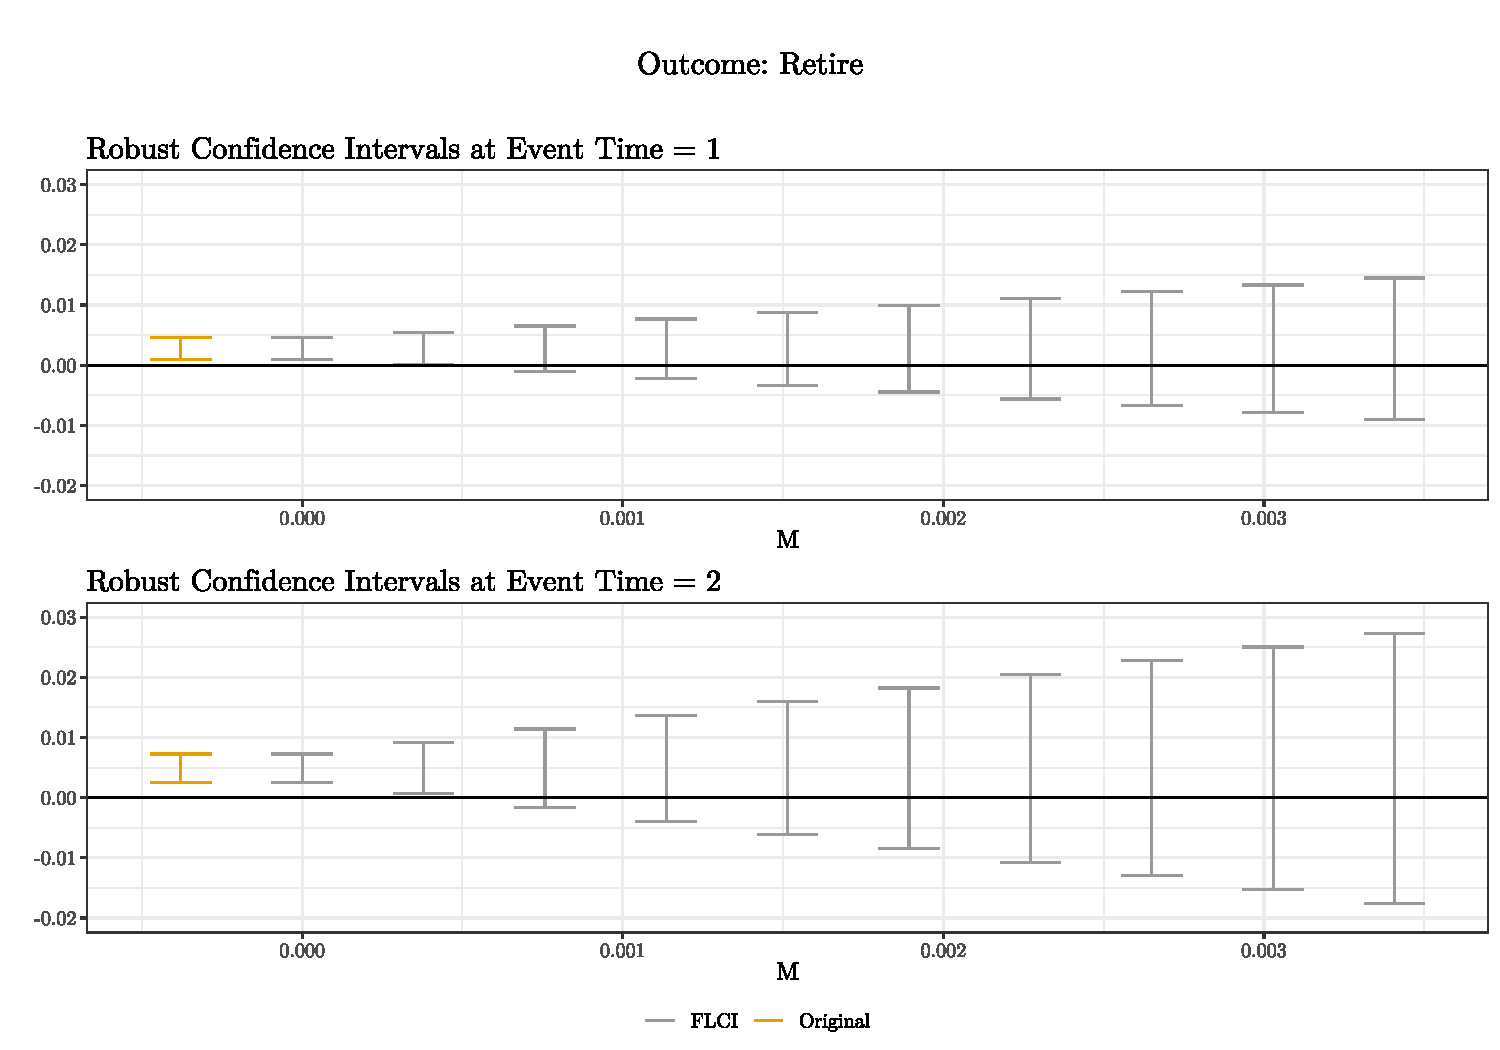
\includegraphics[scale=.5]{Objects/retire_pretrends_plot.pdf}
    \label{fig:pre_retire}
    \vspace{2mm}
    \caption*{\footnotesize{\textit{Notes: This plot shows average treatment effects one year after EHR exposure under different trend assumptions. M=0 indicates a linear pre-trend.}}}
\end{figure}

\subsubsection{Work in Office Likelihood}

Next, I examine pre-trends for the outcome variable indicating whether the physician does any work in an office. The p-values do not indicate pre-trends for the full sample or for physicians $< 60$, but I reject no pre-trends for physicians of retirement age. I show robust confidence intervals for the average treatment effect in the first year after exposure in Figure \ref{fig:pre_work}. For various assumptions on the form of pre-trends, the positive effect holds.

\begin{figure}[ht]
    \centering
    \captionsetup{width=.5\linewidth}
    \caption{Work in Office Indicator}
    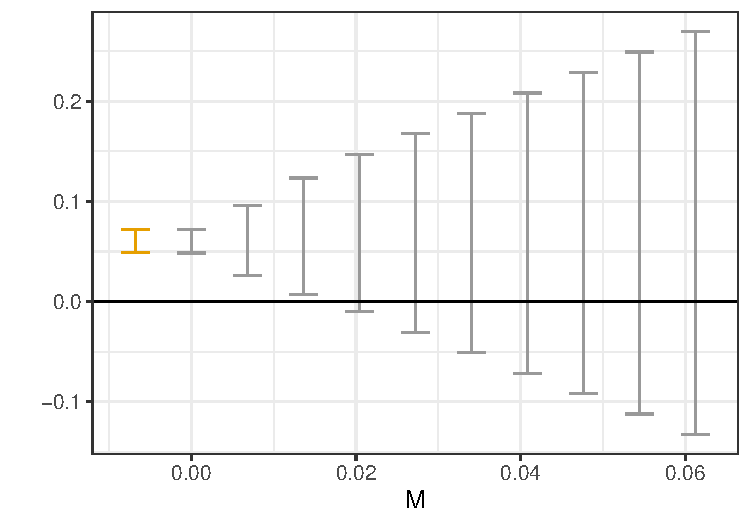
\includegraphics[scale=.5]{Objects/office_ind_pretrends_plot.pdf}
    \label{fig:pre_work}
    \vspace{2mm}
    \caption*{\footnotesize{\textit{Notes: Notes: This plot shows average treatment effects one year after EHR exposure under different trend assumptions. M=0 indicates a linear pre-trend.}}}
\end{figure}

\subsubsection{Fraction of Patients in Office}

The next outcome considered is the fraction of patients seen in an office setting. All p-values suggest there are no pre-trends. I show robust confidence intervals for the average treatment effect in the first year after exposure in Figure \ref{fig:pre_frac}. For various assumptions on the form of pre-trends, the positive effect holds.

\begin{figure}[ht]
    \centering
    \captionsetup{width=.5\linewidth}
    \caption{Fraction of Patients Seen in Office}
    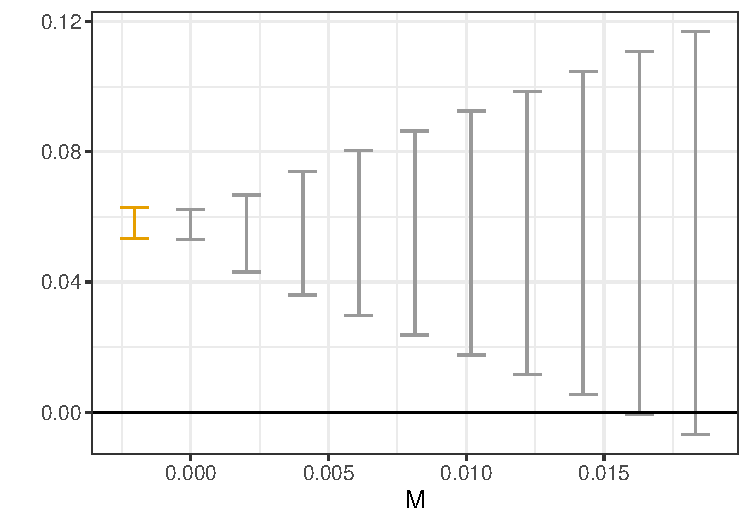
\includegraphics[scale=.5]{Objects/office_frac_pretrends_plot.pdf}
    \label{fig:pre_frac}
    \vspace{2mm}
    \caption*{\footnotesize{\textit{Notes: This plot shows average treatment effects one year after EHR exposure under different trend assumptions. M=0 indicates a linear pre-trend.}}}
\end{figure}

\subsubsection{Patient Count}

Now I examine the sensitivity of the main specification results where the outcome considered is the number of patients seen. None of the p-values indicate a violation of parallel trends, but I present a plot of confidence intervals robust to specified variations in parallel trends as a robustness check in Figure \ref{fig:pre_patient}. This plots indicate that, even under nonlinear deviations in parallel trends, there is a positive effect of EHR exposure on patient count with similar magnitude to that of the main specification.  

\begin{figure}[ht]
    \centering
    \captionsetup{width=.5\linewidth}
    \caption{Patient Count}
    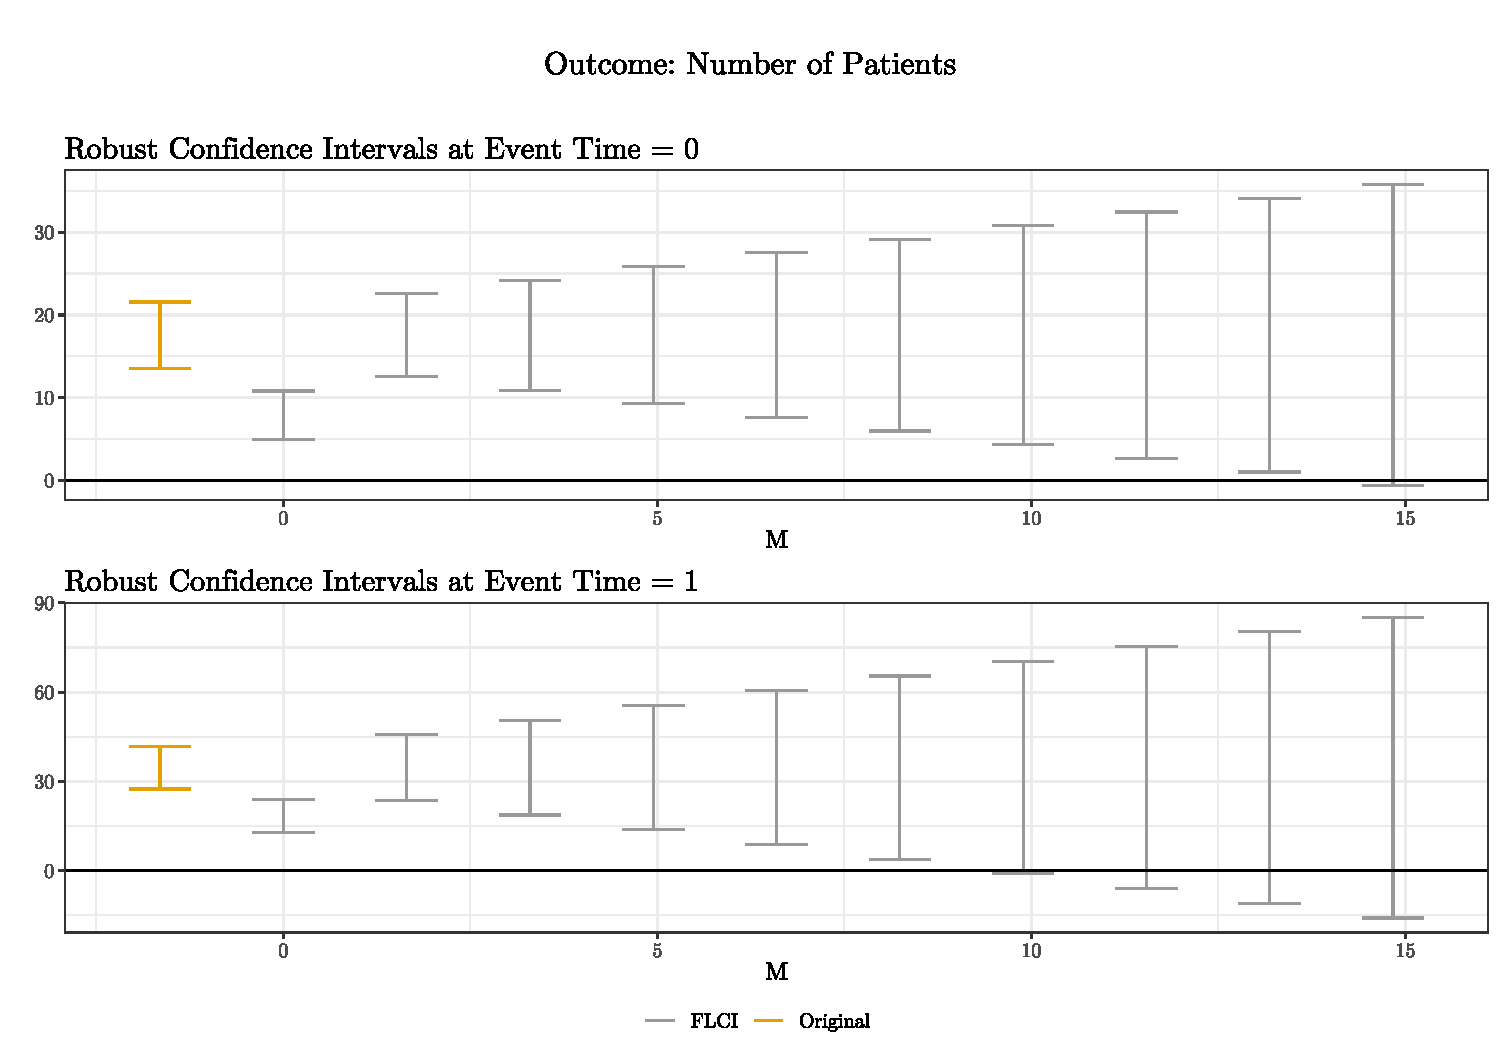
\includegraphics[scale=.5]{Objects/patient_pretrends_plot.pdf}
    \label{fig:pre_patient}
    \vspace{2mm}
    \caption*{\footnotesize{\textit{Notes: This plot shows average treatment effects one year after EHR exposure under different trend assumptions. M=0 indicates a linear pre-trend.}}}
\end{figure}

\subsubsection{Claim Count}

Finally, I assess the results found in the main specification for the outcome variable claim count. The main specification indicates an increase in claims per patient after EHR exposure, but under various specification changes this effect becomes null. Under linear assumptions of a pre-trend form, the effect is similar to that of the main specification. Once more non-linearity is allowed, the effect becomes null. 

\begin{figure}[ht]
    \centering
    \captionsetup{width=.5\linewidth}
    \caption{Claims per Patient}
    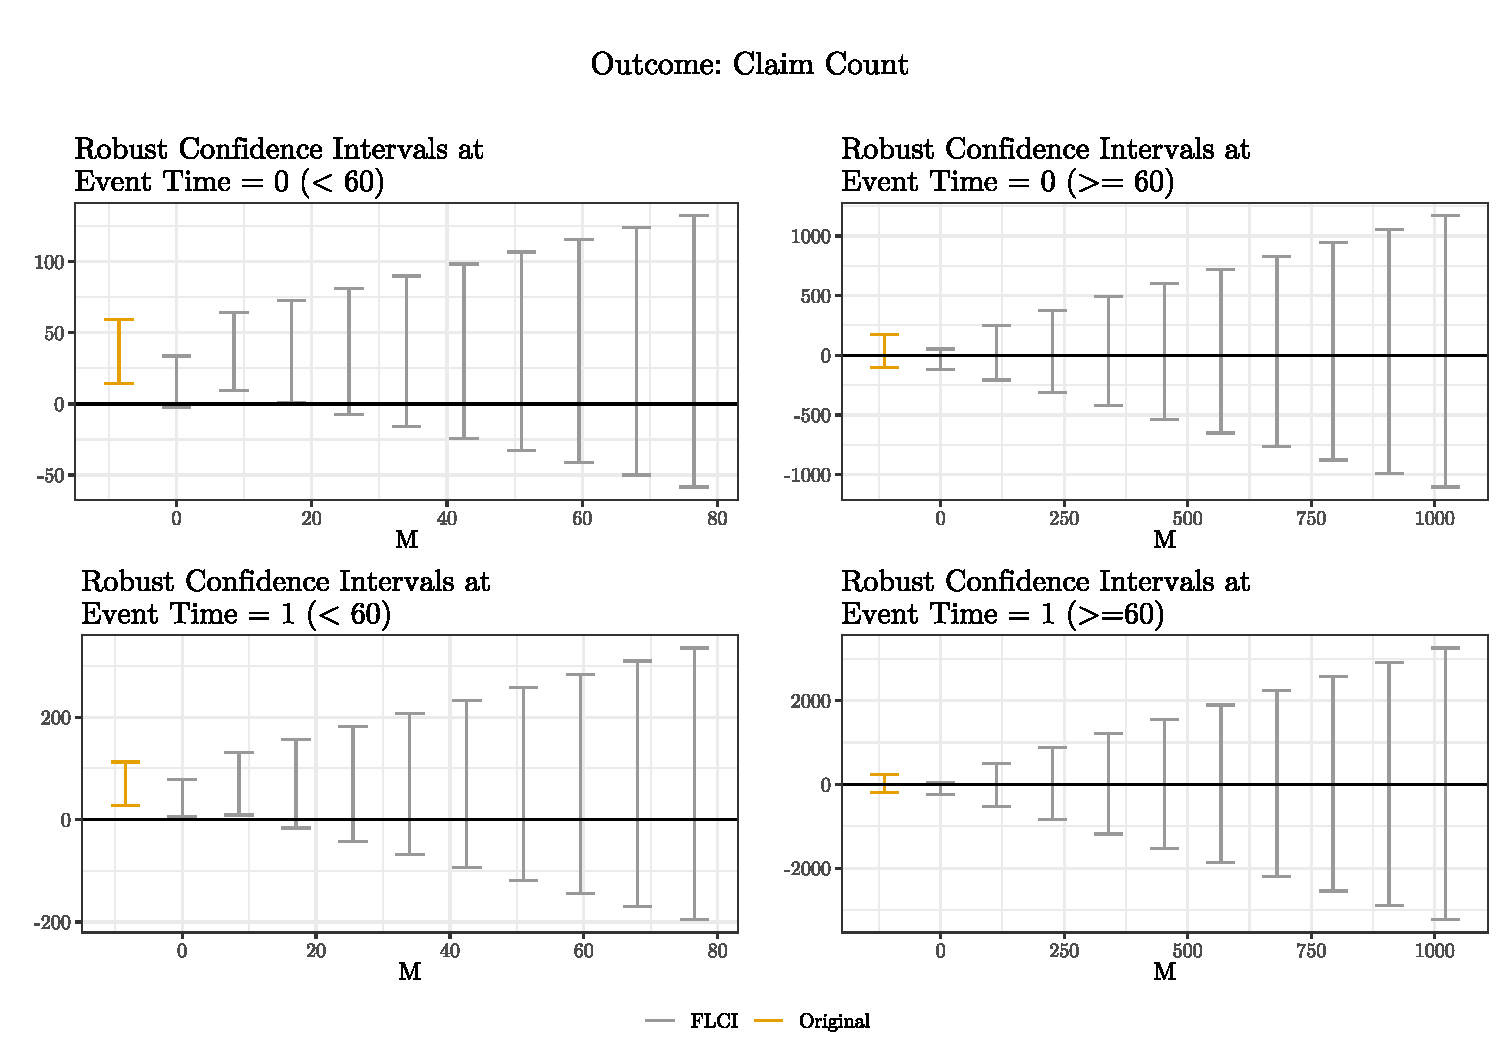
\includegraphics[scale=.5]{Objects/claim_pretrends_plot.pdf}
    \label{fig:pre_claim}
    \vspace{2mm}
    \caption*{\footnotesize{\textit{Notes: This plot shows average treatment effects one year after EHR exposure under different trend assumptions. M=0 indicates a linear pre-trend.}}}
\end{figure}

\subsection{Various Changes to Specification}\label{sec:changes}

For each outcome, there are various adjustments I make to the main specification in order to show robustness. Some of these changes address potential endogeneity concerns, while some provide evidence that the results do not depend on thresholds which may be arbitrary. I will outline each of these adjustments and then present specification charts which account for different combinations of these changes. 

While there is evidence to suggest the time it takes to implement an EHR does not exceed one year, there still may be some anticipation if physicians are expecting implementation in the hospitals they work in. Thus, the specification charts that I present in Section \ref{sec:chart} include specifications where one year of anticipation occurs. 

In the main sample, I define dependent variables using years 2009 to 2017 and drop any physicians who were not exposed to an EHR by 2015 due to data constraints. This leads to estimation based on not yet treated units, because all never treated units are dropped. As a robustness check, I limit sample years to 2009-2015 and use never treated units as the control group. 

There are two main thresholds I define in the data process that were arbitrarily chosen. Thus, I present alternate specifications that adjust these thresholds. First, when deciding which hospitals a physician is working closely with, I drop any pairs that fall below 30 shared patients per year. The goal of this threshold is to eliminate pairs for which the physician does not have close ties to the hospital. In alternate specifications, I lower the threshold to 10 patients per year and raise the threshold to 60 patients per year. Second, I only want to include hospitalists in the analysis, and thus drop any physicians that fall below 70\% of patients in an inpatient setting. In alternate specifications, I change this threshold to 50\% and 90\%. While these are still arbitrary, they provide some evidence that changing the threshold does not dramatically change the results. 


\subsection{Specification Charts}\label{sec:chart}

I present overall average treatment effects for each outcome variable under different combinations of the specification adjustments discussed in Section \ref{sec:changes}. On each chart, the main specification is labeled in green and the average confidence bands across all combinations is shown as an orange band. 

\subsubsection{Leaving Clinical Setting}

The specification chart for the exiting outcome is presented in Figure \ref{fig:retire_chart}. The main specification yields a statistically significant average treatment effect of .0025. This coefficient is on the higher end of coefficients from all combinations of specifications. However, almost all of the coefficients are positive. Some noisy estimates are to be expected when there are multiple limitations placed on the data. These results support the main finding that EHR exposure positively affects the likelihood of leaving a clinical setting among hospitalists. 

\begin{figure}[ht]
    \caption{Outcome: Exit Clinical Setting}
    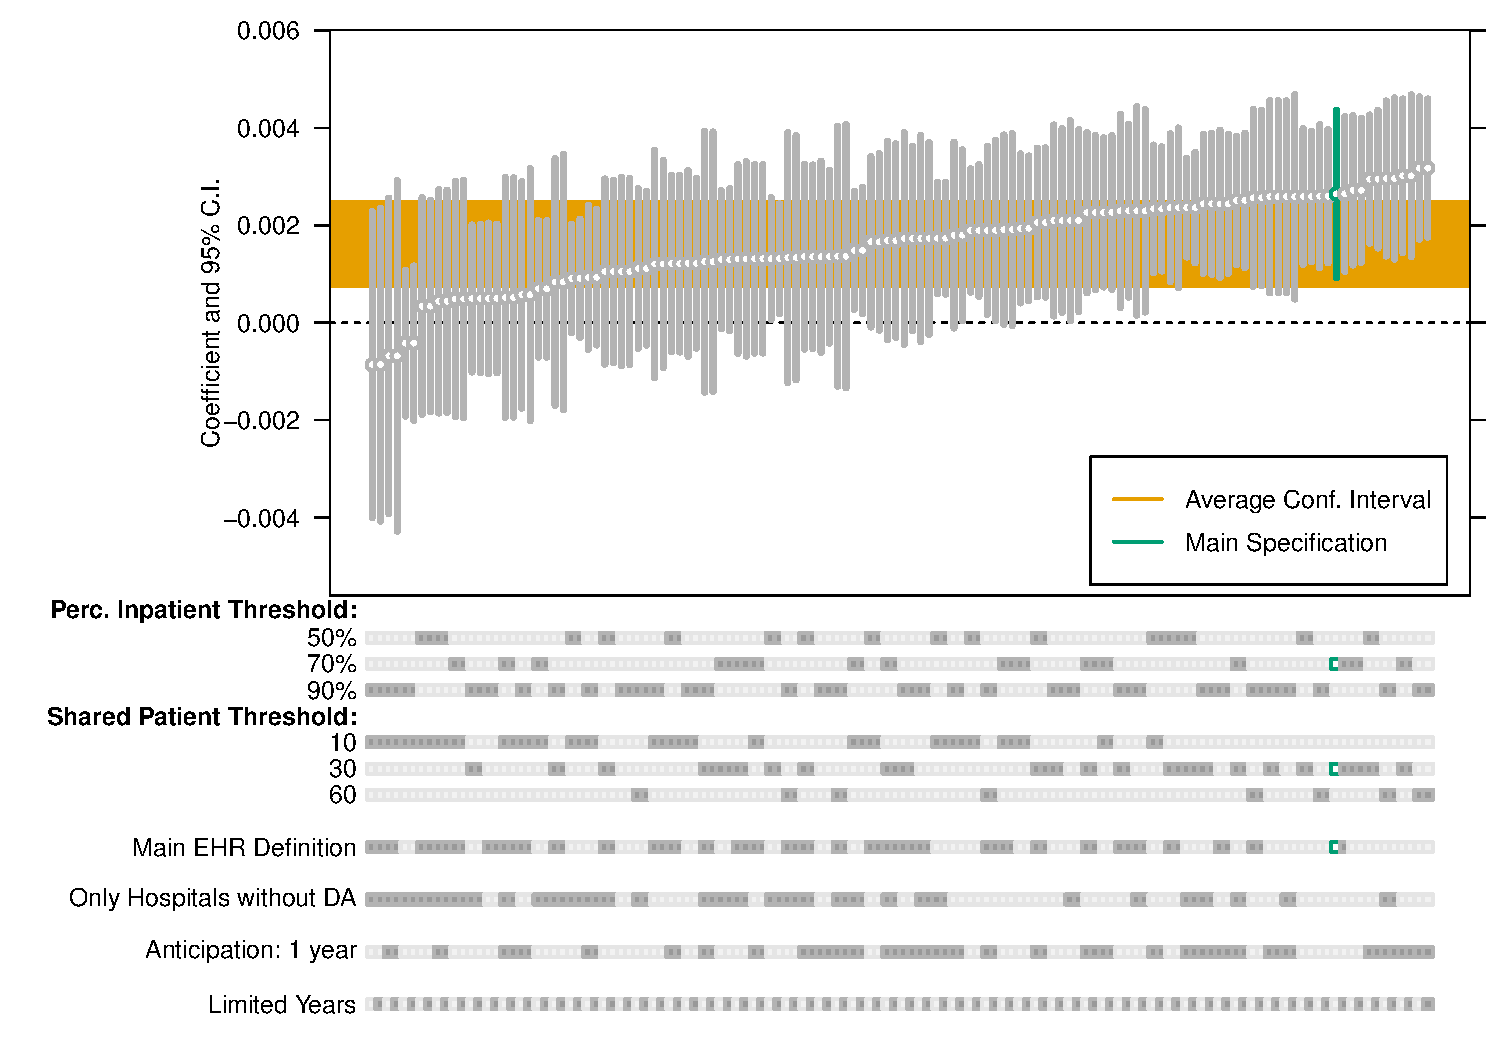
\includegraphics[scale=.7]{Objects/retire_chart.pdf}
    \label{fig:retire_chart}
\end{figure}

\subsubsection{Change Work Setting}

The specification charts for outcomes work in office and fraction of patients seen in office are presented in Figures \ref{fig:work_chart} and \ref{fig:fracoffice_chart}, respectively. First, I discuss the overall average treatment effect of EHR exposure on the likelihood of working in an office. The main specification yields finding that EHR exposure leads to a .07 ppt increase in the likelihood of working in an office. This is on the high end of all combinations of changes to specification, but all reveal a positive effect.   

\begin{figure}[ht]
    \caption{Outcome: Work in Office}
    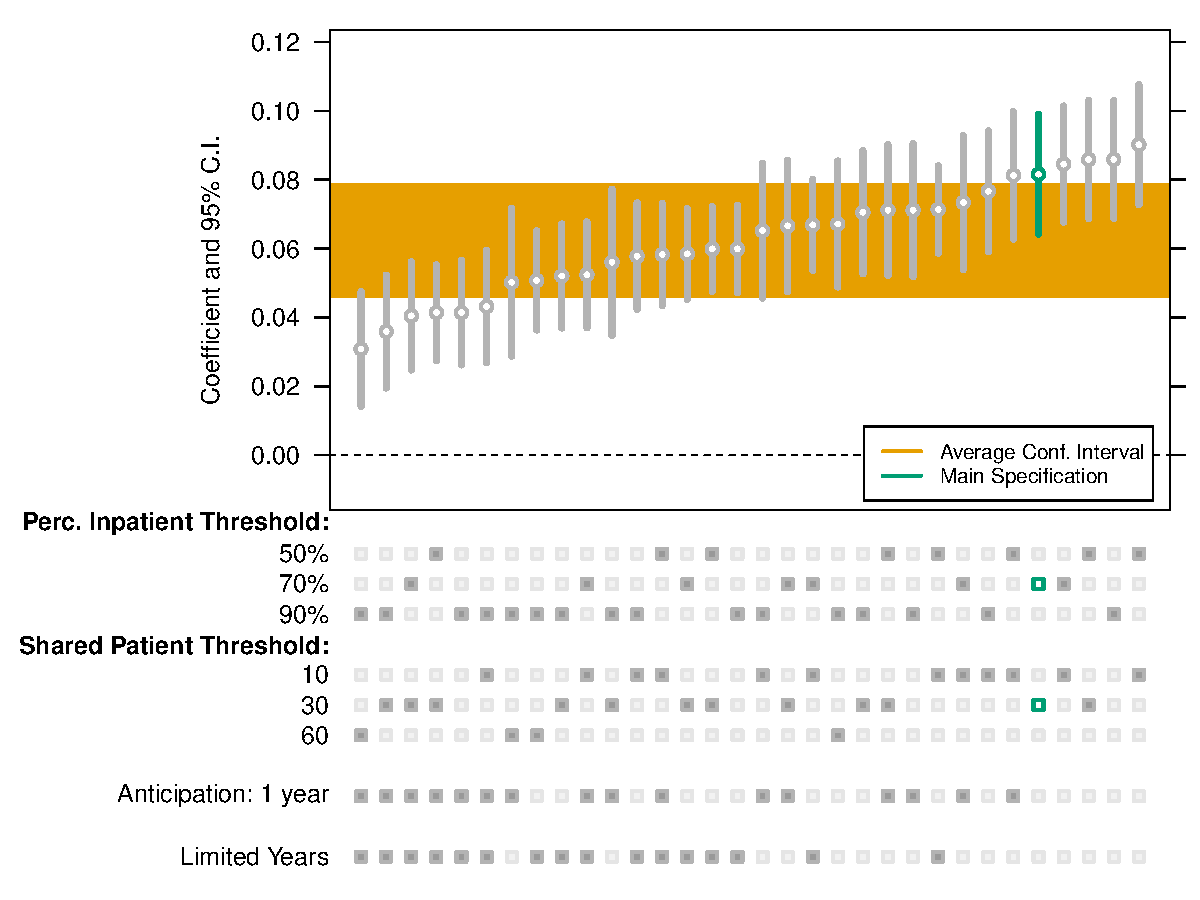
\includegraphics[scale=.7]{Objects/office_ind_chart.pdf}
    \label{fig:work_chart}
\end{figure}

Now I discuss the results for whether hospitalists change the fraction of patients seen in an office setting due to EHR exposure. Similarly, the ATT from the main specification is on the high end of other ATTs found, but all estimates suggest a positive effect. The average of all the confidence intervals found is (.02, .06), suggesting a positive effect on fraction of patients seen in an office. Changes that affect the magnitude of the estimate (but not the sign) are limiting sample years and anticipation. Limiting the years in the sample and allowing for one year of anticipation both push the magnitude of the estimate down. 

\begin{figure}[ht]
    \caption{Outcome: Fraction of Patients in Office}
    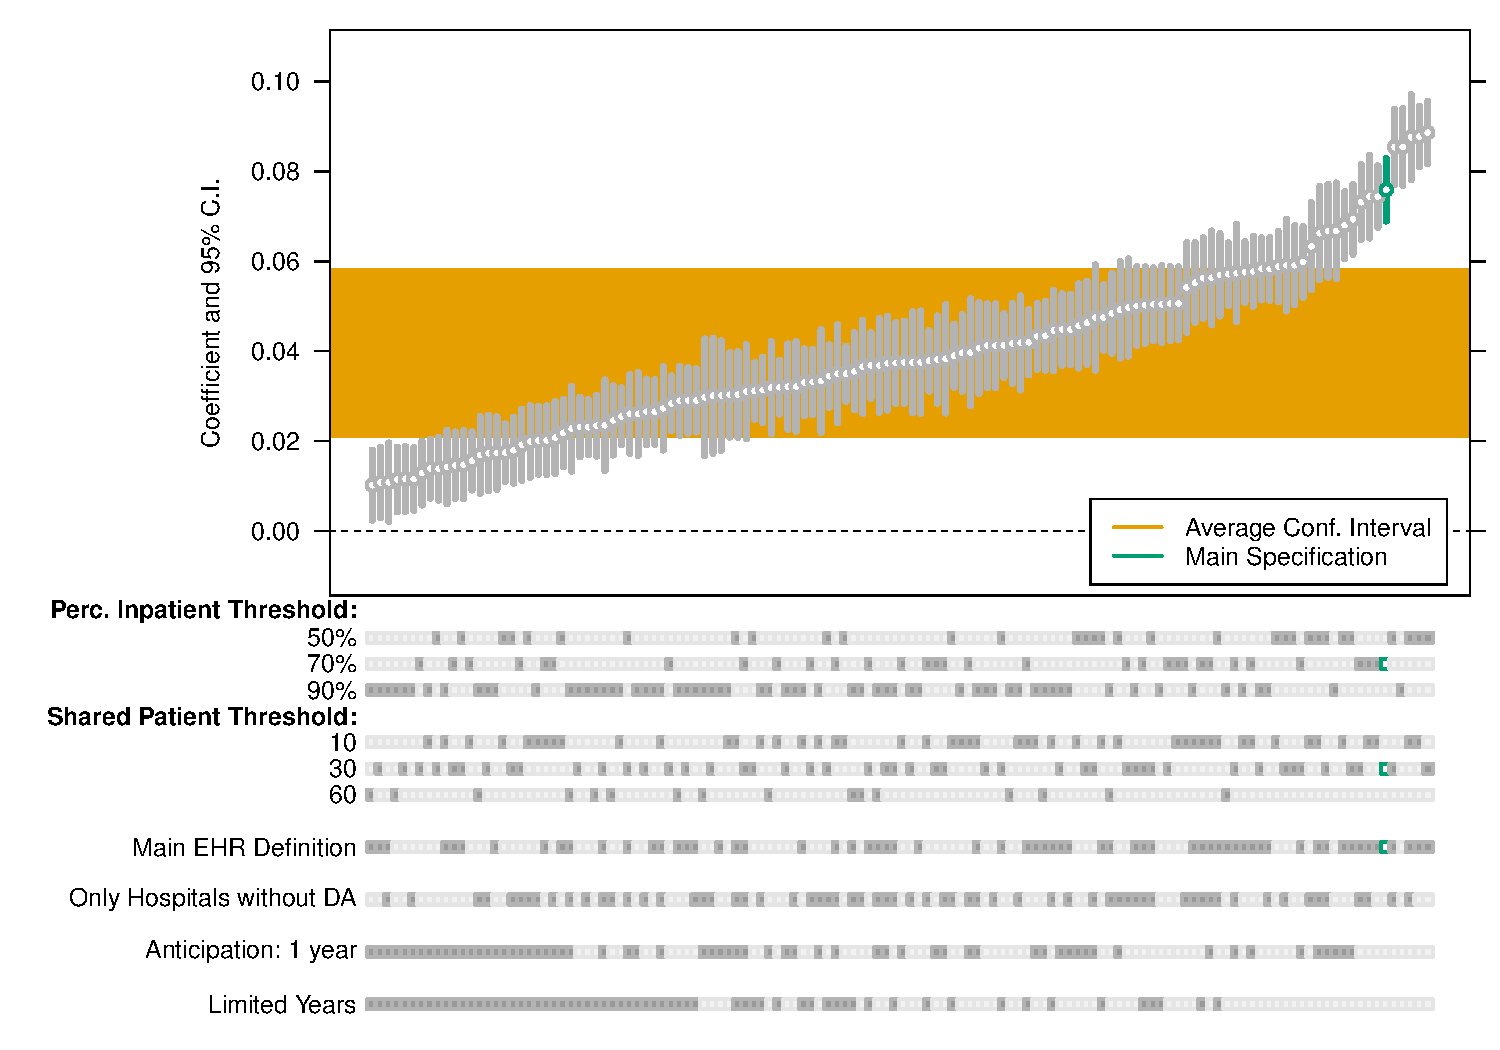
\includegraphics[scale=.7]{Objects/office_frac_chart.pdf}
    \label{fig:fracoffice_chart}
\end{figure}


\subsubsection{Patient Count and Claims per Patient}

In Figure \ref{fig:pat_chart}, I present estimates and confidence intervals for different combinations of specification changes. The result from the main specification is that EHR exposure increases patient count by 28. While most specifications yield positive estimates, about a third of the specifications have a confidence interval that includes zero. It doesn't seem as though any specific change is driving the null result, so I hypothesize that it is due to the reduction in observations due to data limiting. The average of all of the confidence intervals is 7 to 23, indicating that a positive effect on patient count is reasonable. 

\begin{figure}[ht]
    \caption{Outcome: Patient Count}
    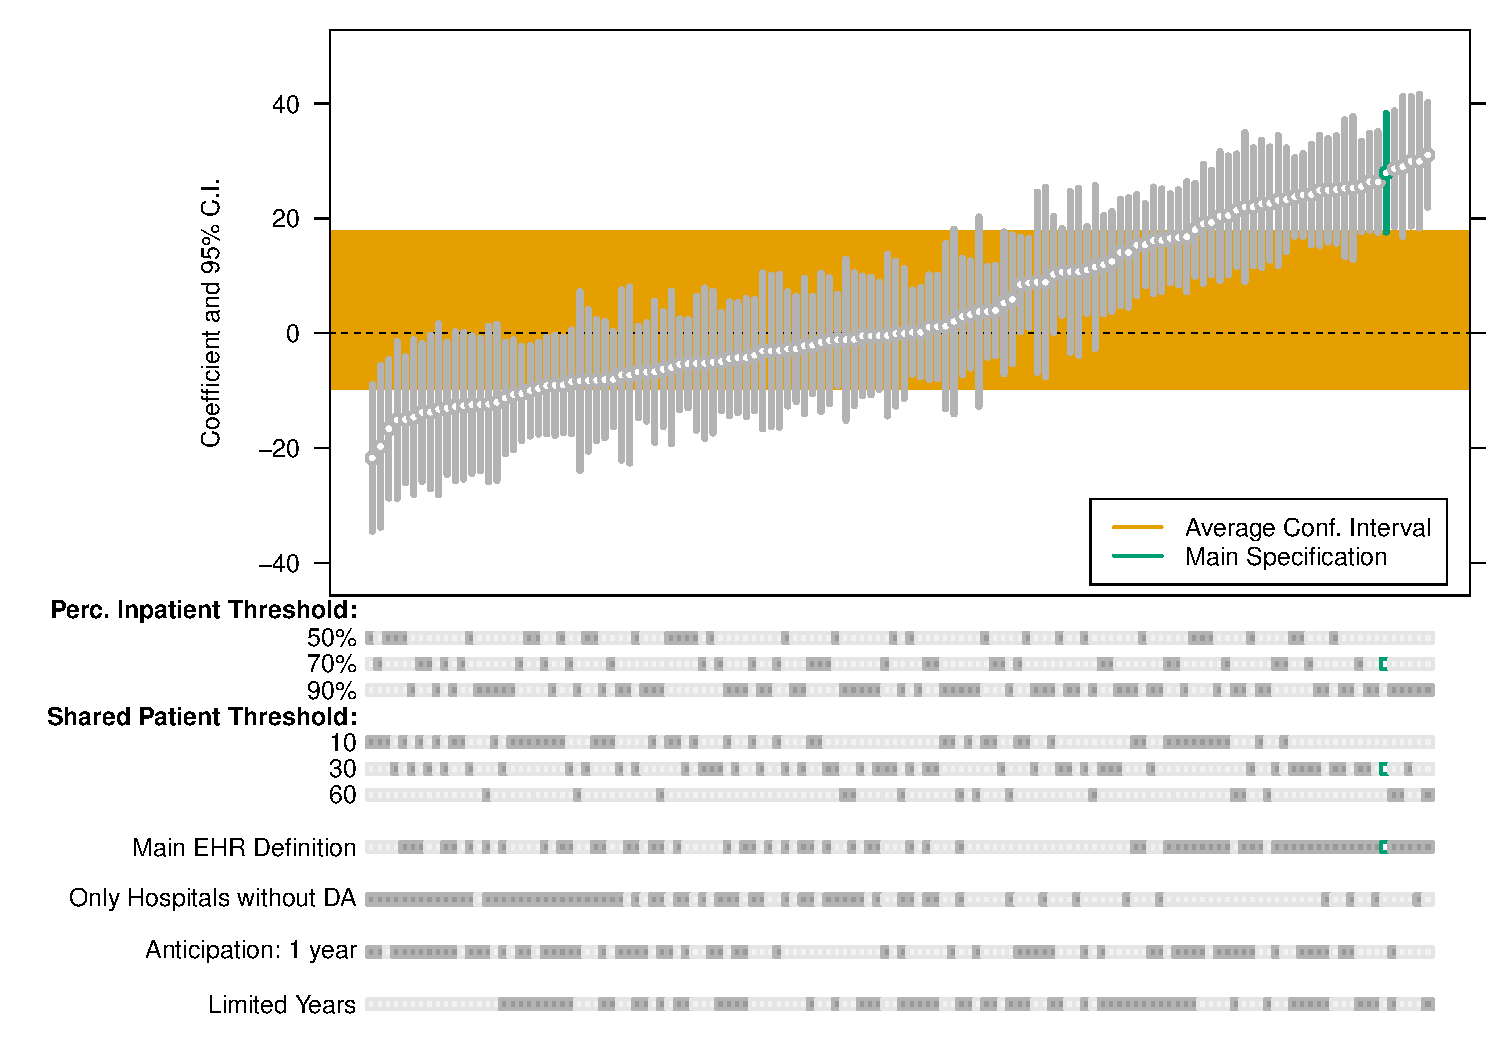
\includegraphics[scale=.7]{Objects/patient_chart.pdf}
    \label{fig:pat_chart}
\end{figure}

Lastly, I examine a chart of estimates for different specifications attempting to capture the effect of EHR exposure on claims per patient. My main finding is that EHR exposure increases claims per patient by around .3. However, various robustness checks reveal that this is overestimated. That is supported in this specification chart as well, where around half of the estimated confidence intervals include zero. Thus, I make no conclusion that EHR exposure increases claims per patient. 

\begin{figure}[ht]
    \caption{Outcome: Claims per Patient}
    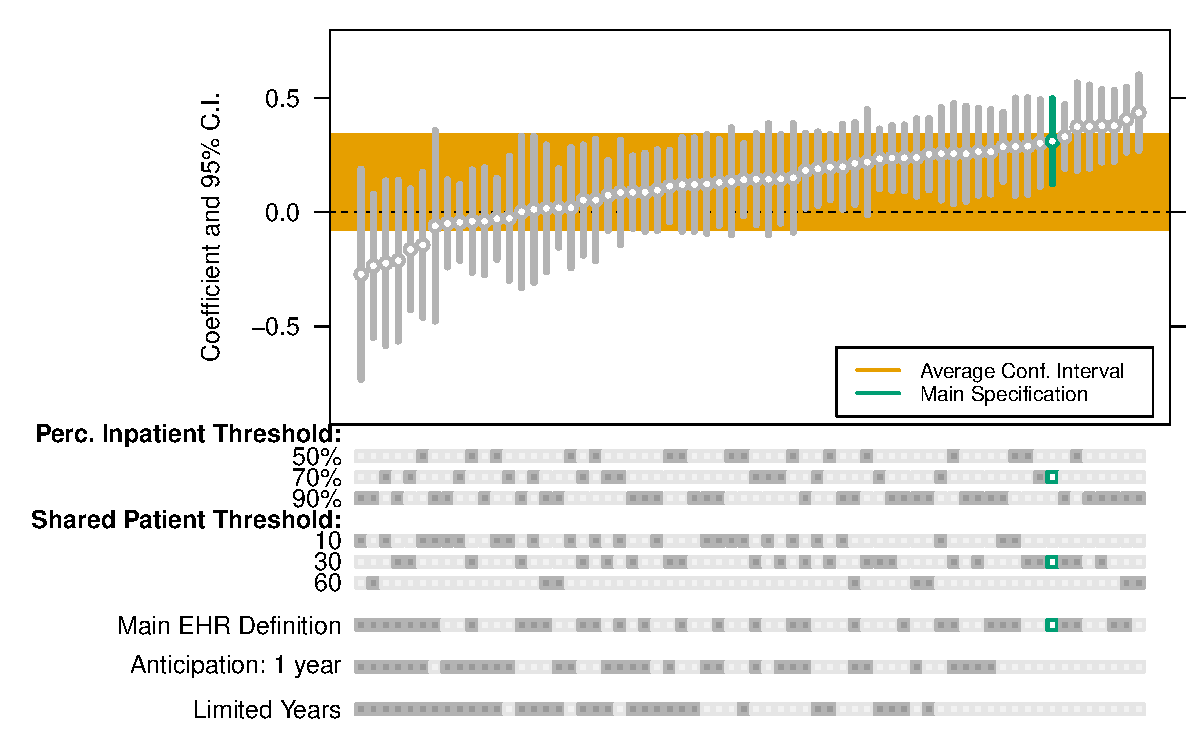
\includegraphics[scale=.7]{Objects/claim_chart.pdf}
    \label{fig:cpp_chart}
\end{figure}

\begin{figure}[ht!]
    \centering
    \captionsetup{width=.6\linewidth}
    \caption{Effect of EHR Exposure on Patient Count by Group}
    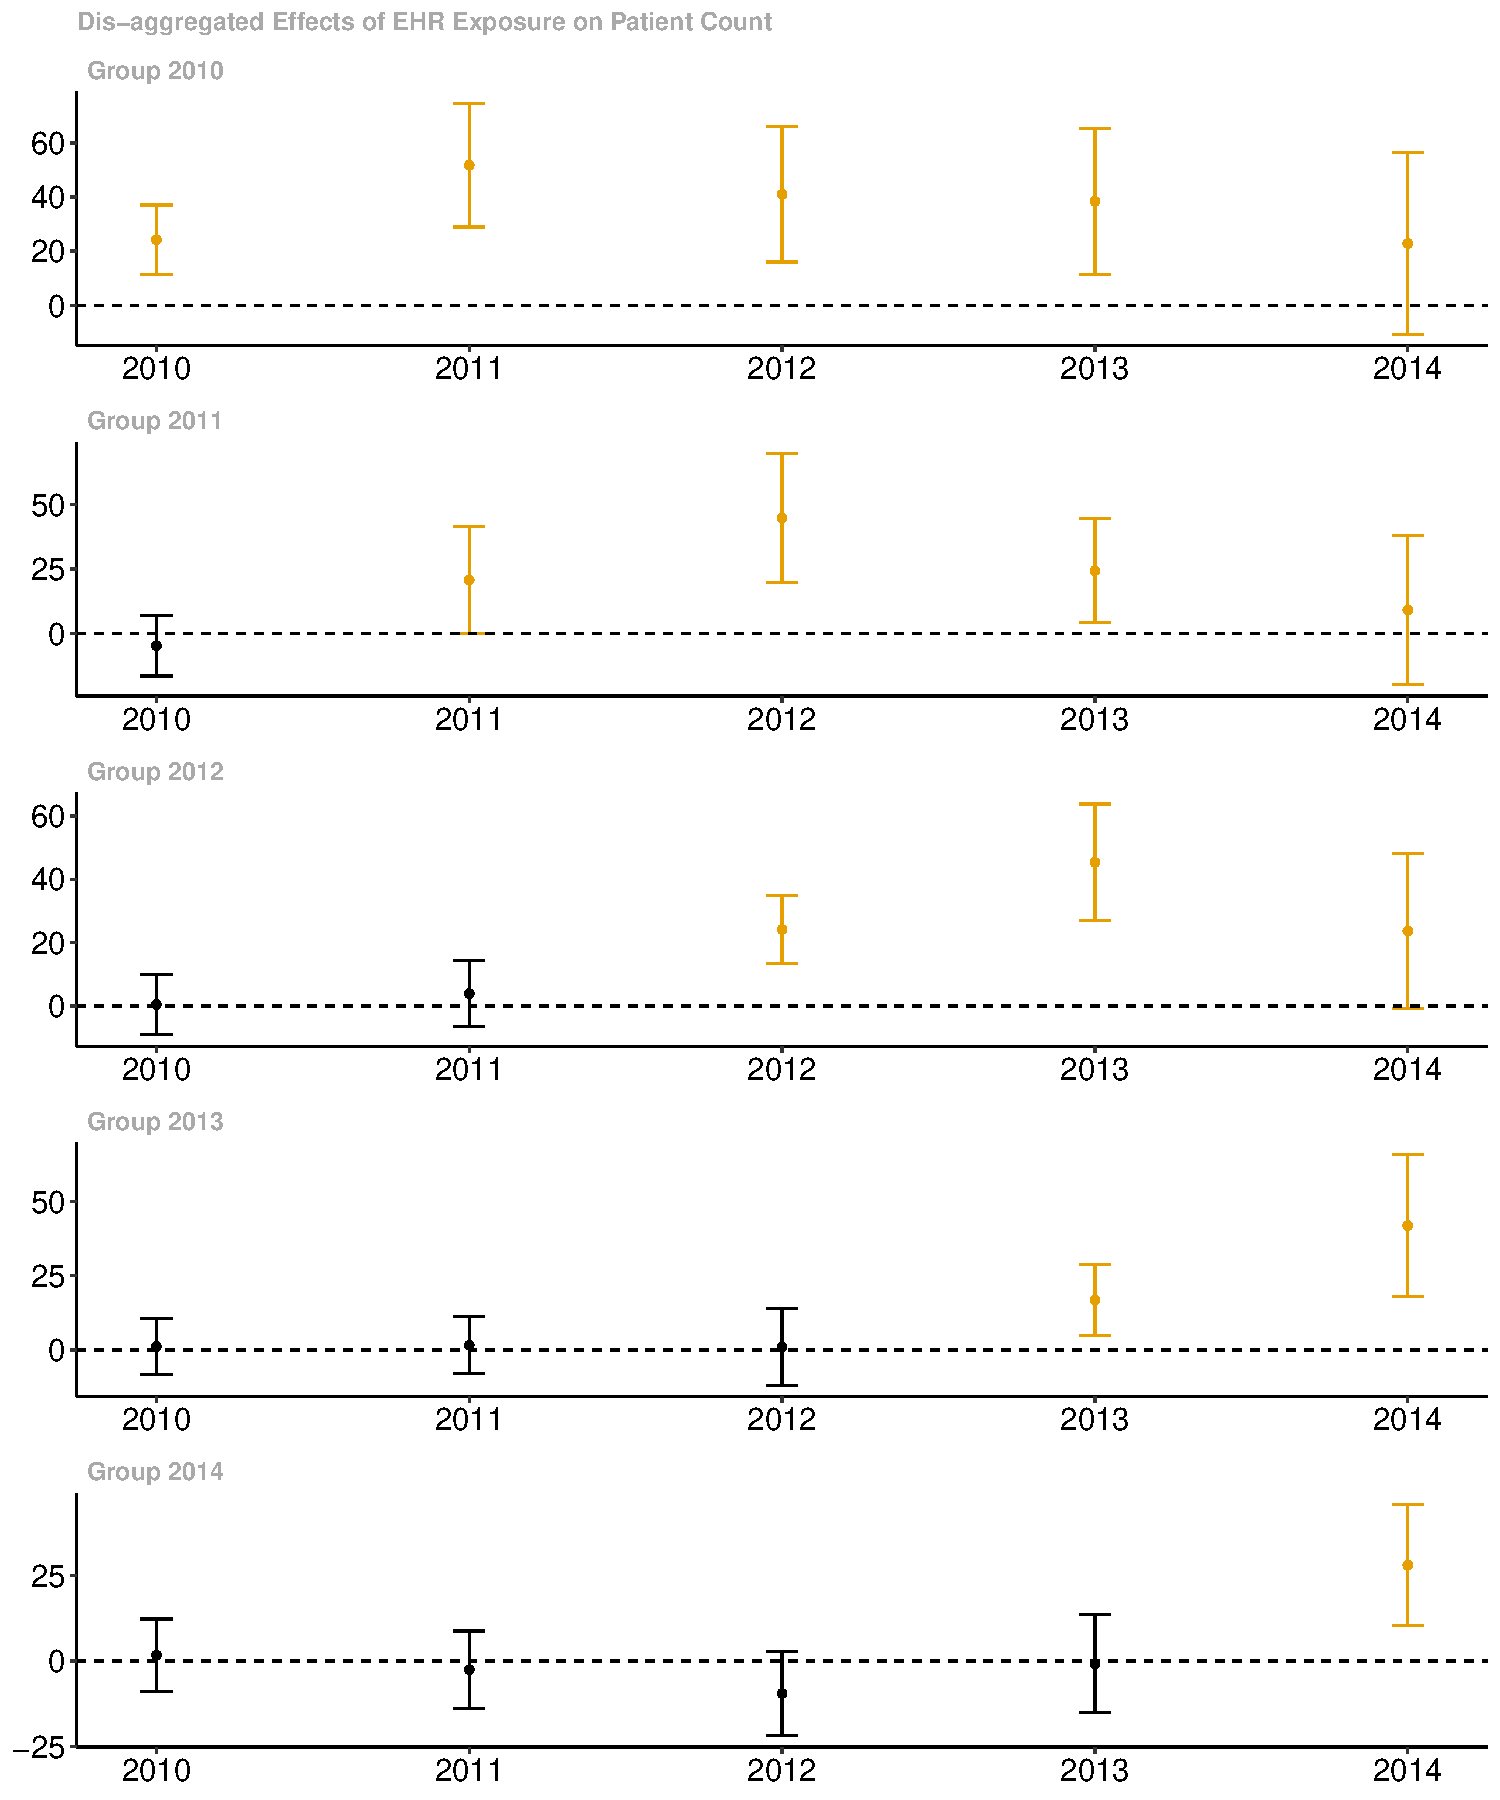
\includegraphics[scale=.4]{Objects/patient_group.pdf}
    \label{fig:patientgroup}
    \vspace{2mm}
    \caption*{\footnotesize{\textit{Notes:} Plot shows average group time treatment effects for each treatment group.}}
\end{figure}





\subsection{Alternative Estimators}\label{app:estimators}

There is a robust recent literature considering the issues with estimating heterogeneous treatment effects with a two way fixed effects specification, the classic approach in staggered treatment setups. To avoid these problems, in my main specification I use the average group time effect estimator established in \citeauthor{callaway2021difference} (\citeyear{callaway2021difference}). In this section, I discuss other potential estimators and why I ultimately included average group time treatment effects as the main specification. 

Before I present these estimators, I present results from a two way fixed effects setup that may suffer bias from negative weighting. Specifically, I estimate the following equation:
$$\text{outcome}_{i,t}=\sum_{j=-4}^{-2} \text{rel\_year}_{j} + \sum_{j=0}^{4} \text{rel\_year}_{j} + \delta_i + \gamma_t,$$
where outcome$_{i,t}$ is one of the five outcomes discussed previously, rel\_year$_j$ is an indicator equal to 1 if year $t$ is $j$ years relative to treatment, $\delta_i$ are physician fixed effects, and $\gamma_t$ are year fixed effects.
These results from each outcome are presented in Figure \ref{fig:twfe}. These results show similar patterns to the main specification, with slight variations in magnitude. 

\begin{figure}
    \centering
    \captionsetup{width=.8\linewidth}
    \caption{Results: Two Way Fixed Effects}
    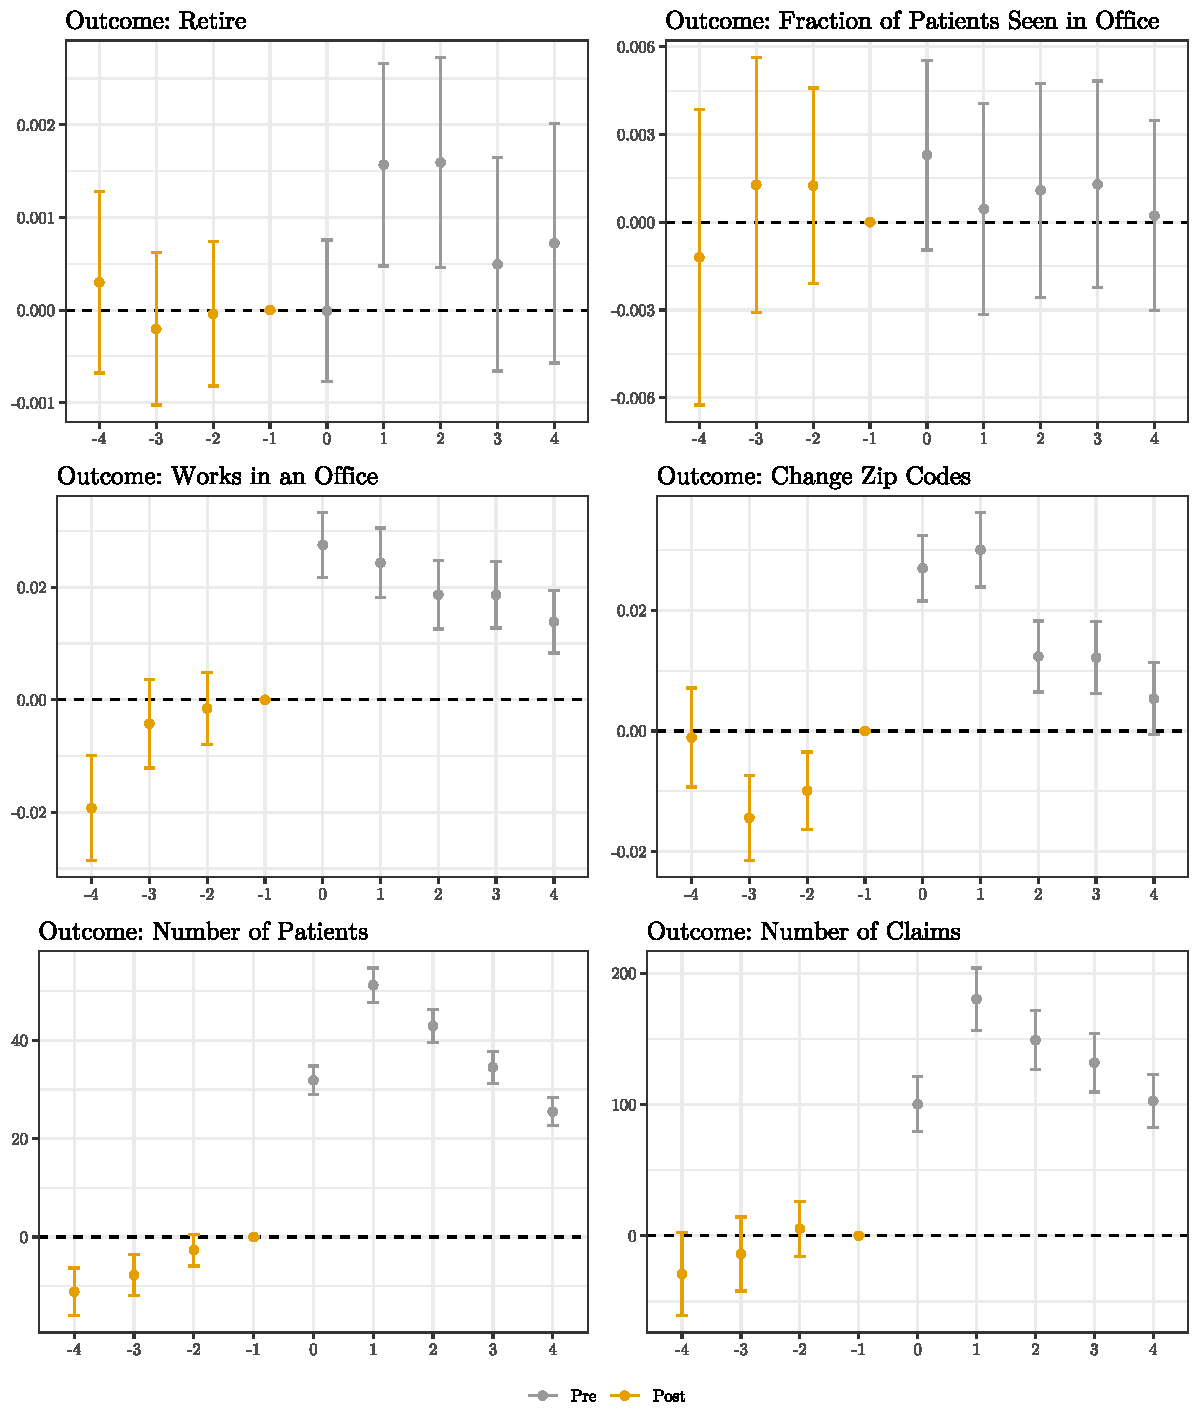
\includegraphics[scale=.6]{Objects/twfe_plot.pdf}
    \label{fig:twfe}
    \vspace{2mm}
    \caption*{\footnotesize{\textit{Notes:} Event study plots from two way fixed effects estimation are shown for each outcome variable.}}
\end{figure}

One method that addresses issues with the TWFE specification by differencing out fixed effects is established in \citeauthor{gardner2021two} (\citeyear{gardner2021two}). This approach is commonly known as two stage difference in differences and is very clever. However, the approach requires a group of never-treated units as the comparison group, a drawback for my study in that I remove all never-treated units to utilize all years of MD-PPAS data, and because never-treated hospitals are likely compositionally different from those treated in the majority of the sample. Nevertheless, I limit the years of data to 2009-2015 and present estimates as a percentage of the mean of each variable in Figure \ref{fig:estimators}. Generally, the results have the same sign with a slightly larger magnitude, driven by the inclusion of never-treated units. 

\begin{figure}
    \centering
    \caption{Alternative Estimators}
    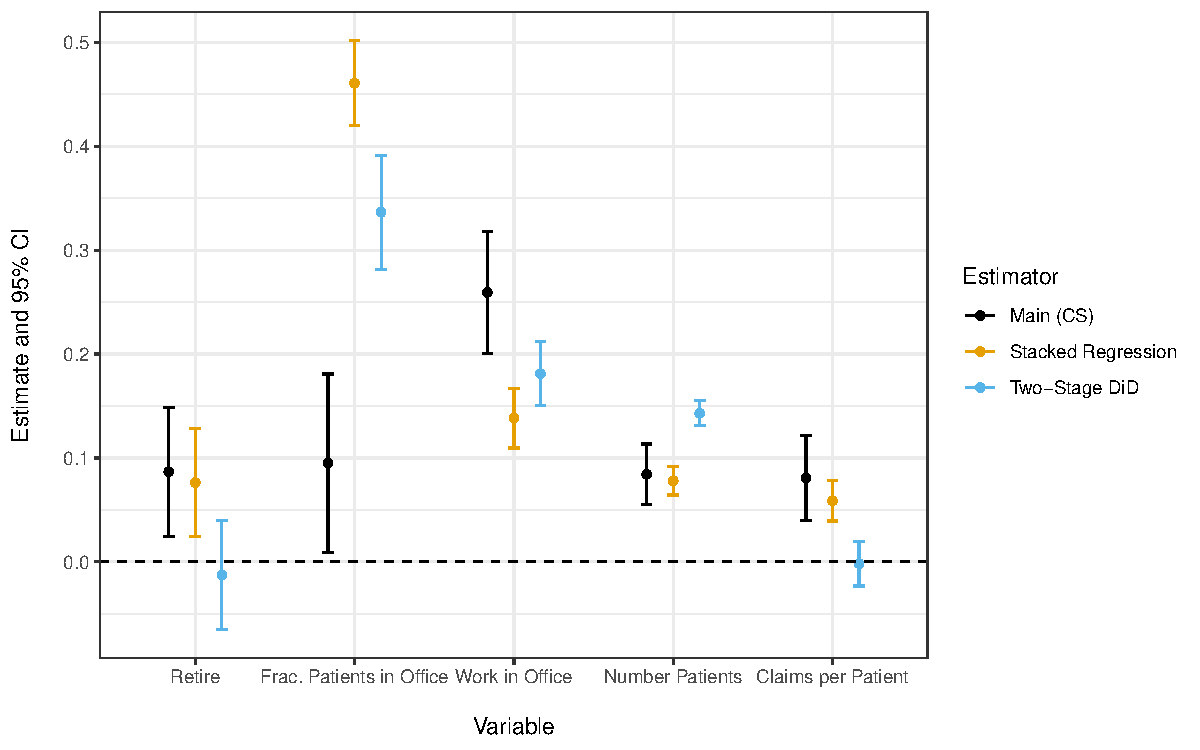
\includegraphics[scale=.6]{Objects/estimators_plot.pdf}
    \label{fig:estimators}
\end{figure}

Another estimation method first used by \citeauthor{cengiz2019effect} (\citeyear{cengiz2019effect}) is commonly known as stacked regression. In this method, one re-frames event study data into groups of sub-experiments that are then stacked on top of each other, defining a group of treated units and ``clean" control units. The drawback of this method is choosing an event study window that must be the same for each treatment group, where a large window eliminates many treated units and a small window does not allow for estimation over many years. I present the results using this method with an event window of one year in Figure \ref{fig:estimators}. The results are very similar to the main specification, with a smaller magnitude in some cases. 





\section{Heterogeneity Analysis}

The main analysis focuses on the differential effects of technology for older vs. younger physicians. However, another important question is whether physicians in rural vs. urban settings respond differently to the technology since the implications for behavior changes are high in areas that already suffer from access to care issues. Thus, I present average treatment effects for each outcome where the sample is split between physicians in rural and urban areas. Further, to investigate the same idea, I present results for physicians who typically work at small hospitals vs. large hospitals. These average treatment effects as a percentage of the mean of each variable are shown in Figure \ref{fig:heter}. The results do not differ along these dimensions. This is fascinating in that technology is creating these adverse effects across completely different practice environments.


\begin{figure}
    \centering
    \caption{Heterogeneity Analysis}
    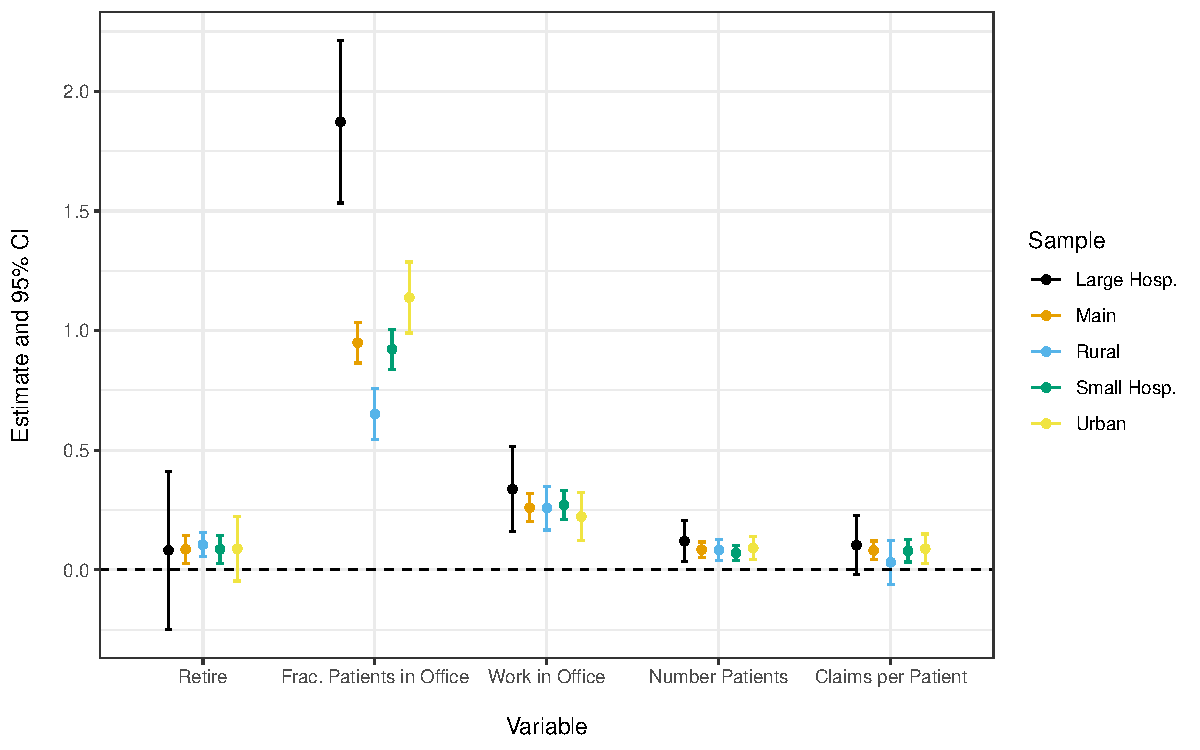
\includegraphics[scale=.6]{Objects/heterog_plot.pdf}
    \label{fig:heter}
\end{figure}




















\end{document}